\chapter{DESAIN DAN IMPLEMENTASI}
\label{chap:desainimplementasi}


\section{Struktur Rencana Kerja Pengembangan (WBS)}
\sloppy
Penelitian ini menggunakan pendekatan pengembangan berbasis \emph{Work Breakdown Structure} (WBS), yaitu metode sistematis untuk membagi keseluruhan proses pengembangan ke dalam unit-unit kerja yang lebih kecil dan terstruktur. WBS mencakup tahapan analisis kebutuhan, perancangan, implementasi, hingga evaluasi, yang disusun secara hierarkis untuk memudahkan perencanaan dan pelaksanaan sistem secara efisien. Diagram WBS yang digunakan dalam penelitian ini dapat dilihat pada Gambar \ref{fig:wbs}.

\begin{figure}[H]
  \centering
  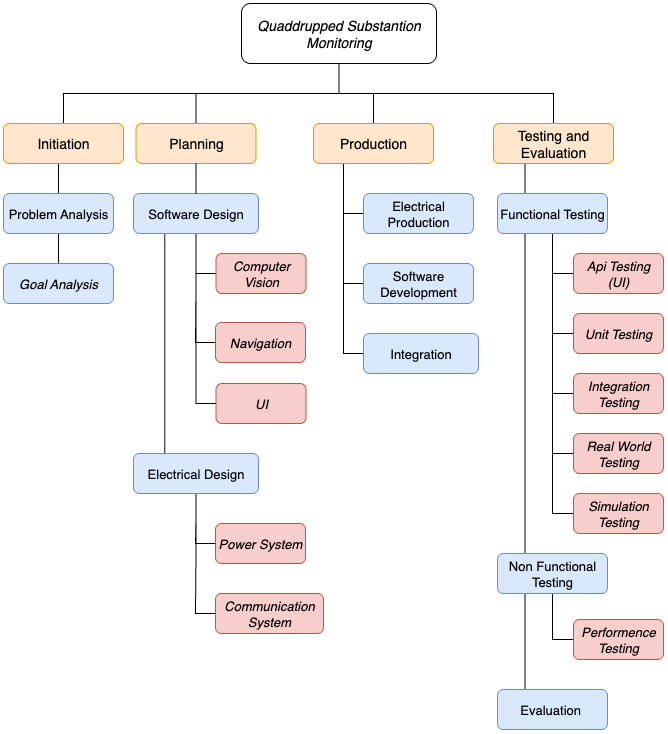
\includegraphics[width=0.85\textwidth]{gambar/bab3/wbs-ta.png}
  \caption{\emph{Work Breakdown Structure} (WBS) Penelitian}
  \label{fig:wbs}
  \footnotesize{\textbf{Sumber:} Penulis}
\end{figure}

\section{Desain Pengembangan Sistem}
Pengembangan dalam penelitian ini bertujuan untuk melakukan otomatisasi proses pemantauan suhu komponen gardu induk yang sebelumnya dilakukan secara manual, dengan memanfaatkan robot berkaki empat \emph{(quadruped-legged)} Deep Robotics X30 Pro. Agar sistem mampu melakukan pemantauan secara otomatis, diperlukan pengembangan lebih lanjut dari kondisi robot yang ada saat ini. Pengembangan sistem ini mencakup tiga tujuan utama, yaitu: sistem deteksi suhu komponen, sistem navigasi otonom, dan sistem \emph{control station}. Melalui pengembangan ini, diharapkan robot dapat melakukan patroli secara mandiri di area gardu induk, mendeteksi komponen yang mengalami kondisi \emph{overheat}, serta menyampaikan informasi yang relevan kepada operator melalui sistem \emph{control station}. Dalam proses pengembangan ini selain dilakukan pengembangan perangkat lunak robot, juga dilakukan integrasi perangkat keras tambahan seprti kamera termal, modul komunikasi nirkabel, dan perangkat lunak sebagai sistem \emph{control station} yang akan digunakan untuk memantau kondisi robot dan memberikan informasi terkait potensi \emph{overheat} secara \emph{real-time}.

\subsection{Desain Elektrikal}

Desain elektrikal robot mencakup perancangan sistem distribusi daya dan komunikasi yang bertujuan untuk mengintegrasikan komponen-komponen tambahan ke dalam sistem robot yang telah ada. Komponen tambahan ini dirancang untuk mendukung kapabilitas operasi otonom robot secara menyeluruh. Rancangan lengkap dari sistem dapat dilihat pada Gambar~\ref{fig:electrical}.

\begin{figure}[H]
  \centering
  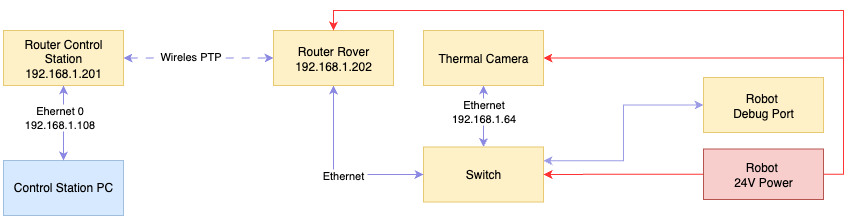
\includegraphics[width=0.85\textwidth]{gambar/bab3/electrical-design.png}
  \caption{Desain Elektrikal Robot}
  \label{fig:electrical}
  \footnotesize{\textbf{Sumber:} Dokumentasi Pribadi}
\end{figure}

Pada Gambar~\ref{fig:electrical}, ditunjukkan bahwa robot dilengkapi dengan sejumlah komponen tambahan guna mendukung fungsi pemantauan suhu secara otomatis. Komponen-komponen tersebut antara lain meliputi kamera termal Hikvision HM-TD5528T-15/W, router Doublecom DB6000FR-ANS, dan perangkat \emph{switch} jaringan. Seluruh perangkat tambahan ini memerlukan catu daya sebesar 24~VDC yang disuplai langsung dari port daya pada \emph{navigation host} robot, sehingga tidak memerlukan sumber daya eksternal tambahan. Dari sisi komunikasi internal, seluruh perangkat jaringan di dalam robot terhubung melalui \emph{switch} jaringan yang kemudian diintegrasikan ke dalam sistem utama robot melalui \emph{debug port}. Konfigurasi ini membentuk suatu jaringan lokal tertutup \emph{(closed local network)}. Untuk mendukung komunikasi eksternal antara robot dan sistem \emph{control station}, digunakan skema komunikasi nirkabel \emph{Point-to-Point} (PTP) pada frekuensi 5{,}8~GHz. Dalam konfigurasi ini, perangkat pemancar yang terpasang pada \emph{control station} (Doublecom DB6000ANLT90-FR) dikonfigurasi sebagai \emph{access point} (AP), sedangkan perangkat penerima yang berada pada sisi robot berfungsi sebagai \emph{station}. Skema ini memungkinkan terjadinya pertukaran data dua arah berkecepatan tinggi dengan latensi rendah, yang sangat krusial untuk mendukung transmisi data secara \emph{real-time}, 


\subsection{Desain Sistem \emph{Computer Vision}}

Sistem \emph{computer vision} yang dikembangkan bertujuan untuk mendeteksi jenis komponen gardu induk serta menganalisis suhunya guna mengidentifikasi potensi \emph{overheat}. Proses ini dilakukan melalui tiga tahap utama, yaitu ekstraksi suhu dari citra termal, deteksi objek menggunakan model \emph{YOLO}, dan pemetaan intensitas ke suhu aktual. Langkah pertama adalah memperoleh data suhu maksimum dari citra termal menggunakan protokol \emph{ISAPI (Intelligent Security API)}. Jika suhu maksimum pada frame melampaui ambang batas minimum potensi \emph{overheat} berdasarkan data suhu overheat terkecil dari komponen dalam basis data, maka dilanjutkan ke tahap deteksi objek. Pendekatan ini dilakukan sebagai optimasi untuk menghindari pemrosesan seluruh citra menggunakan model deteksi, sehingga mengurangi beban komputasi. 

Deteksi objek pada citra termal dilakukan menggunakan model \emph{YOLOv8}, model ini dipilih karena kemampuannya dalam melakukan deteksi objek secara akurat dan cepat. Hal ini penting agar suhu tinggi yang terdeteksi benar-benar berasal dari komponen gardu, dan bukan objek lain di latar. Jika terdapat objek yang dideteksi, maka dilakukan konversi citra termal ke citra skala abu-abu (\emph{grayscale}) untuk memungkinkan pemetaan suhu berdasarkan intensitas piksel. Pemetaan suhu dilakukan dengan mengubah nilai intensitas piksel citra \emph{grayscale} menjadi nilai suhu aktual berdasarkan data suhu minimum dan maksimum yang diperoleh melalui ISAPI. Rumus konversi dari intensitas piksel ke suhu aktual adalah sebagai berikut:

\begin{equation}
T_p = T_{\text{min}} + \left( \frac{I_p - I_{\text{min}}}{I_{\text{max}} - I_{\text{min}}} \right) \cdot (T_{\text{max}} - T_{\text{min}})
\end{equation}

\noindent dengan:
\begin{itemize}
    \item $T_p$ = Suhu pada piksel $p$,
    \item $T_{\text{min}}, T_{\text{max}}$ = Suhu minimum dan maksimum dari ISAPI,
    \item $I_p$ = Nilai intensitas piksel $p$ (0–255),
    \item $I_{\text{min}}, I_{\text{max}}$ = Nilai intensitas minimum dan maksimum pada citra \emph{grayscale}.
\end{itemize}

Nilai suhu aktual dari area pada \emph{bounding box} hasil deteksi objek kemudian dibandingkan dengan ambang batas suhu berdasarkan jenis komponen. Jika melebihi batas tersebut, sistem menyimpulkan adanya potensi \emph{overheat}.





\subsection{Desain Perangkat Lunak Robot}
Desain perangkat lunak pada robot dilakukan dengan mempertimbangkan arsitektur perangkat lunak yang bersifat modular dan terintegrasi. Pendekatan ini bertujuan untuk mempermudah proses pengembangan, pemeliharaan, serta pengujian sistem secara menyeluruh. Dalam penelitian ini, perangkat lunak dibagi menjadi beberapa \textit{package} ROS yang masing-masing memiliki fungsi spesifik dan saling terhubung.

Terdapat empat \textit{package} utama yang dikembangkan, yaitu \textit{IO package}, \textit{Localization and Mapping package}, \textit{Autonomy package}, dan \textit{Perception package}. Struktur umum dari arsitektur perangkat lunak ini dapat dilihat pada Gambar~\ref{fig:software-arch}.

\begin{figure}[H]
  \centering
  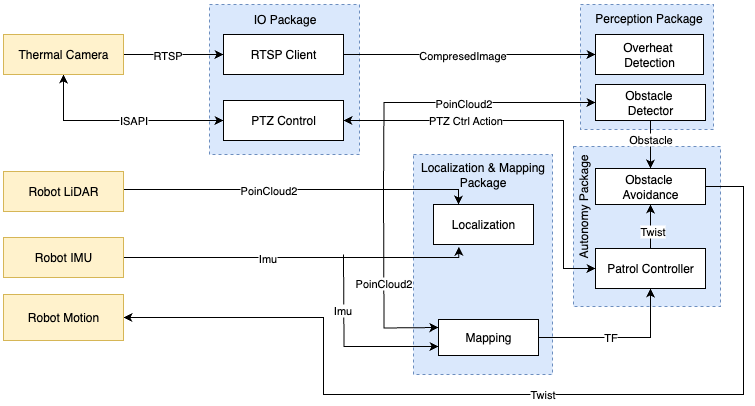
\includegraphics[width=0.8\textwidth]{gambar/bab3/sotware-arch.png}
  \caption{Arsitektur Perangkat Lunak Robot}
  \label{fig:software-arch}
  \footnotesize{\textbf{Sumber:} Dokumentasi Pribadi}
\end{figure}

Setiap \textit{package} menjalankan fungsi tertentu dan saling berkomunikasi melalui mekanisme \textit{topic}, \textit{service}, atau \textit{action} sesuai dengan kebutuhan sistem.

\subsubsection{3.3.3.1 \emph{IO Package}}
\textit{IO package} bertanggung jawab untuk mengelola seluruh input dan output dari perangkat keras robot, yang dalam hal ini adalah kamera thermal. \textit{IO package} terdiri dari dua program utama, yaitu \textit{RTSP client} dan \textit{PTZ controller}.  \textit{RTSP client} berfungsi untuk menghubungkan kamera thermal dengan sistem robot dan mengubah aliran data menjadi \textit{rostopic} berupa \textit{compressed image}. Sementara itu, \textit{PTZ controller} digunakan untuk mengatur pergerakan \textit{pan-tilt-zoom} (PTZ) serta menerima status posisi PTZ saat ini menggunakan protokol ISAPI. Informasi ini kemudian digunakan untuk mengontrol pergerakan PTZ secara dinamis, yang dipadukan dengan \textit{PID controller} untuk memperoleh kecepatan rotasi dan sudut target yang akurat.

\subsubsection{3.3.3.2 \emph{Localization and Mapping Package}}
\emph{Localization and Mapping Package} bertanggung jawab untuk melakukan estimasi posisi robot secara \emph{real-time} di dalam lingkungan serta memperbarui peta berdasarkan data sensor yang diterima. Dalam penelitian ini, sistem memanfaatkan empat buah sensor LiDAR Livox Mid-360 dan satu unit Yesense-IMU sebagai sumber data utama. Sistem ini mengimplementasikan berbagai metode \emph{localization} yang mencakup pendekatan berbasis \emph{odometry-only} maupun pendekatan berbasis \emph{Simultaneous Localization and Mapping} (SLAM). Dua metode pertama merupakan metode berbasis \emph{odometry-only}, yaitu \emph{FastLIO2} dan \emph{DLIO} (\emph{Direct LiDAR-Inertial Odometry}), yang melakukan estimasi posisi robot secara langsung berdasarkan integrasi data LiDAR dan IMU tanpa melakukan pemetaan lingkungan. Karena tidak membentuk peta, metode ini memiliki keterbatasan dalam hal inisialisasi di mana proses \emph{localization} harus selalu dimulai dari posisi awal yang sama setiap kali sistem dijalankan, sehingga tidak adaptif terhadap perubahan posisi awal robot. 

Metode ketiga dan keempat menggunakan konsep pemisahan antara proses \emph{mapping} dan \emph{localization} yang tetap terintegrasi sesuai prinsip \emph{frontend-backend} dalam sistem SLAM modern. Pada metode ketiga proses pemetaan dilakukan menggunakan \emph{FastLIO2} untuk menghasilkan representasi peta dua dimensi dalam bentuk \emph{grid-map}, yang kemudian dimanfaatkan oleh \emph{HDL Localization} untuk melakukan proses pelokalan. Pendekatan keempat menggunakan metode \emph{Fast-LIO-SAM} yang menggabungkan estimasi \emph{LiDAR-Inertial Odometry} (LIO) pada \emph{frontend} dengan proses optimisasi graf berbasis \emph{Smoothing and Mapping} (SAM) pada \emph{backend}, menghasilkan peta lingkungan tiga dimensi dalam format file \texttt{.bag} yang kemudian digunakan oleh \emph{Fast-LIO Localization QN} untuk proses \emph{localization}. Pada metode ketiga dan keempat, proses \emph{mapping} dan \emph{localization} tidak berjalan secara bersamaan sehingga memerlukan peta hasil pemetaan yang telah tersedia sebelum proses \emph{localization} dijalankan. Koordinat posisi robot yang dihasilkan dipublikasikan ke dalam sistem ROS melalui transformasi koordinat menggunakan modul \emph{tf broadcaster}.

\subsubsection{3.2.3.1 \emph{Perception Package}}
\emph{Perception package} bertanggung jawab untuk melakukan estimasi posisi komponen yang mengalami panas berlebih (\emph{overheat}) pada gardu induk. Proses ini dilakukan dengan meimplementasikan sistem \emph{computer vision} yang telah dijelaskan pada subbab 3.2.1.  Selain itu \emph{Perception package} juga mengelola deteksi rintangan yang dilakukan oleh robot. Sistem ini menggunakan algoritma \emph{Braitenberg} untuk mendeteksi dan menghindari rintangan di sekitar robot. Deteksi rintangan dilakukan dengan memanfaatkan sensor LiDAR yang terpasang pada robot, yang menghasilkan garis deteksi rintangan dalam sudut 180 derajat dari sisi kiri ke arah depan robot. Setiap garis deteksi memiliki bobot atau nilai \emph{multiplier} yang berbeda, yang digunakan untuk menilai tingkat risiko dan menentukan keputusan gerakan robot. Hasil  deteksi rintangan, akan diteruskan ke \emph{autonomy package} sebagai masukan untuk pengambilan keputusan navigasi secara otonom. Dengan pendekatan ini, sistem mampu melakukan deteksi serta identifikasi objek secara efisien, dan memberikan kontribusi penting dalam memastikan keselamatan serta efektivitas pergerakan robot di lingkungan nyata.

\subsubsection{3.2.3.2 \emph{Autonomy Package}}
Dalam sistem \emph{autonomy}, yang pada dasarnya merupakan proses navigasi jalur, lintasan robot diperoleh dari hasil perekaman \emph{path} yang dilakukan pada saat proses pemetaan. Jalur ini kemudian disimpan dalam format \texttt{.json}. pada database \emph{control station}. Integrasi antara pengendalian lintasan dan penghindaran rintangan menjadi aspek yang krusial dalam sistem ini. Salah satu strategi yang umum digunakan adalah mengimplementasikan algoritma \emph{PID Pure Pursuit} sebagai pengendali utama lintasan, sementara modul penghindaran rintangan berbasis \emph{Braitenberg} diaktifkan secara kondisional ketika objek terdeteksi dalam jarak tertentu. Pendekatan ini memungkinkan robot untuk tetap mengikuti jalur yang telah direkam, namun tetap mampu bereaksi secara dinamis terhadap rintangan tanpa harus melakukan perencanaan ulang lintasan secara menyeluruh. Integrasi semacam ini dapat direalisasikan melalui skema \emph{behavior-based arbitration} atau \emph{subsumption architecture}, di mana modul penghindaran rintangan memiliki prioritas lebih tinggi ketika kondisi kritis terdeteksi. Setelah lingkungan kembali aman, kontrol akan dialihkan kembali ke pengendali lintasan utama. Selain navigasi jalur \emph{autonomy package} juga mengelola proses pengambilan gambar dari kamera termal yang terpasang pada robot. Proses ini dilakukan jika robot telah sampai pada titik koordinat tertentu yang telah ditentukan sebelumnya sistem akan mengirim perintah ke \emph{IO package} untuk mengerakan kamera termal ke posisi yang telah ditentukan. Setelah kamera berada pada posisi yang tepat, \emph{IO package} akan mengirim perintah ke \emph{RTSP client} untuk mengambil gambar dimana gambar yang diambil akan dikirim ke \emph{perception package} untuk dilakukan deteksi objek dan analisis suhu. 

\subsection{Desain \textit{Control Station}}
Sistem ini dirancang layaknya sebuah \emph{fleet management system} yang bertugas untuk memantau dan mengatur seluruh aktivitas operasional robot di lapangan secara \emph{real-time}. Fungsi utama dari sistem ini mencakup pemantauan posisi robot secara langsung pada peta, penyajian hasil deteksi suhu komponen serta visualisasi potensi \emph{overheat} pada komponen gardu, akses terhadap tampilan kamera langsung (\emph{live camera}), serta pengaturan dan penjadwalan jalur patroli.  Perancangan \emph{control station} ini mengadopsi pendekatan berbasis web. Proses perancangan melibatkan beberapa tahapan diantaranya.

\subsubsection{3.2.4.1 Perancangan \emph{User Interface}}
 Tahap ini mencakup desain visual antarmuka, termasuk tata letak, elemen grafis, dan skema warna. Tujuannya adalah menciptakan antarmuka yang  intuitif dan mudah digunakan. Desain UI harus mempertimbangkan aspek estetika sekaligus fungsionalitas, sehingga pengguna dapat dengan mudah memahami dan mengoperasikan sistem. Berikut adalah desain antarmuka \emph{control station} yang telah dirancang:

\begin{figure}[H]
  \centering
  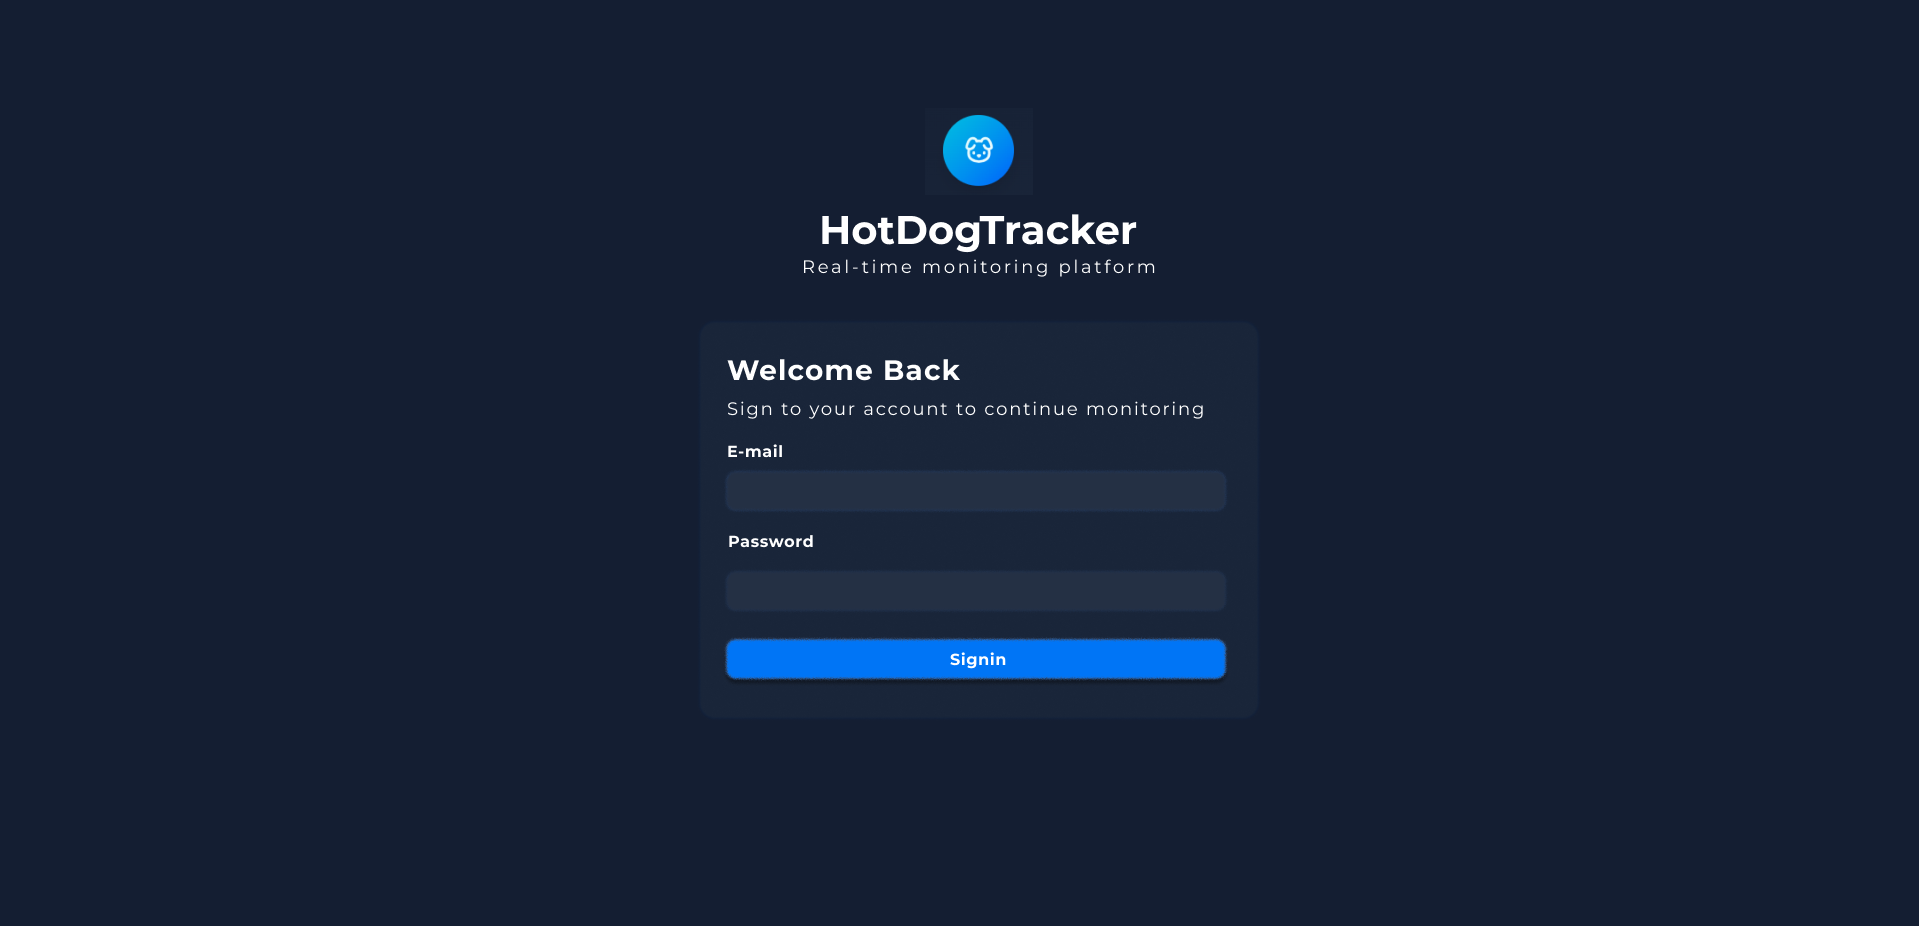
\includegraphics[width=0.8\textwidth]{gambar/bab3/auth-ui.png}
  \caption{Desain halaman login \emph{control station}}
  \label{fig:control-station-auth}
  \footnotesize{\textbf{Sumber:} Dokumentasi Pribadi}
\end{figure}


\begin{figure}[H]
  \centering
  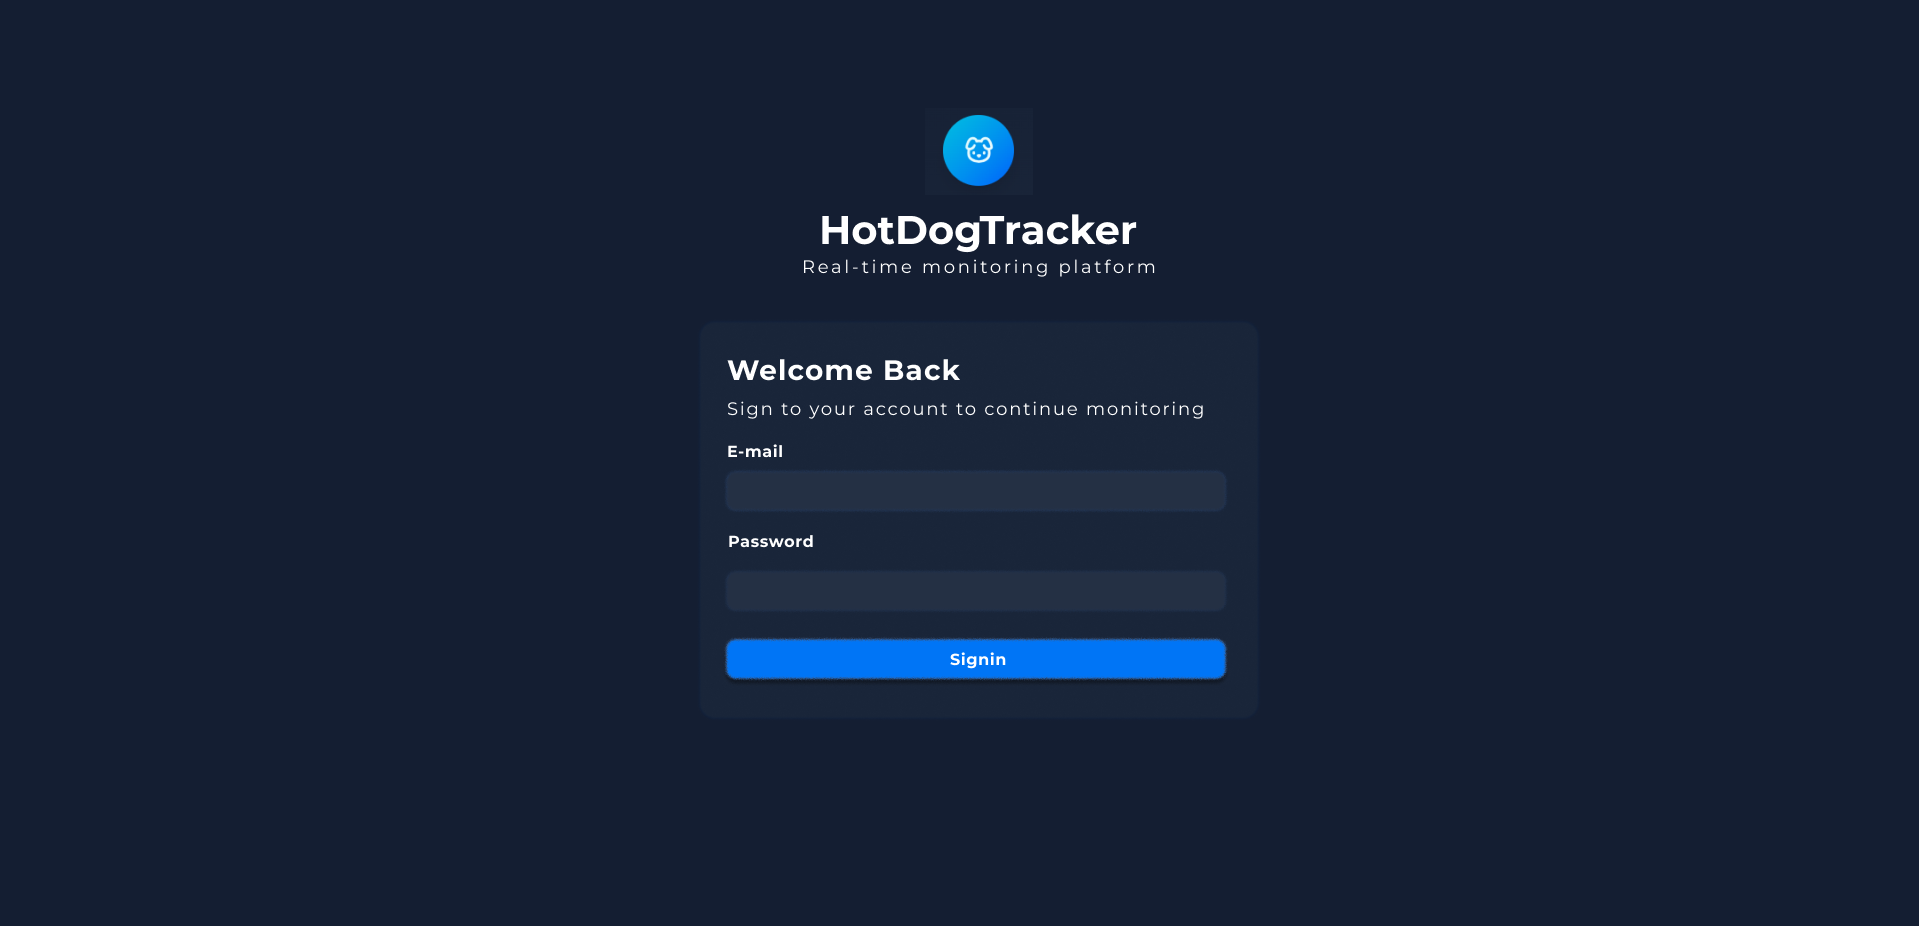
\includegraphics[width=0.8\textwidth]{gambar/bab3/auth-ui.png}
  \caption{Desain halaman utama \emph{control station}}
  \label{fig:control-station-robot-main}
  \footnotesize{\textbf{Sumber:} Dokumentasi Pribadi}
\end{figure}

\begin{figure}[H]
  \centering
  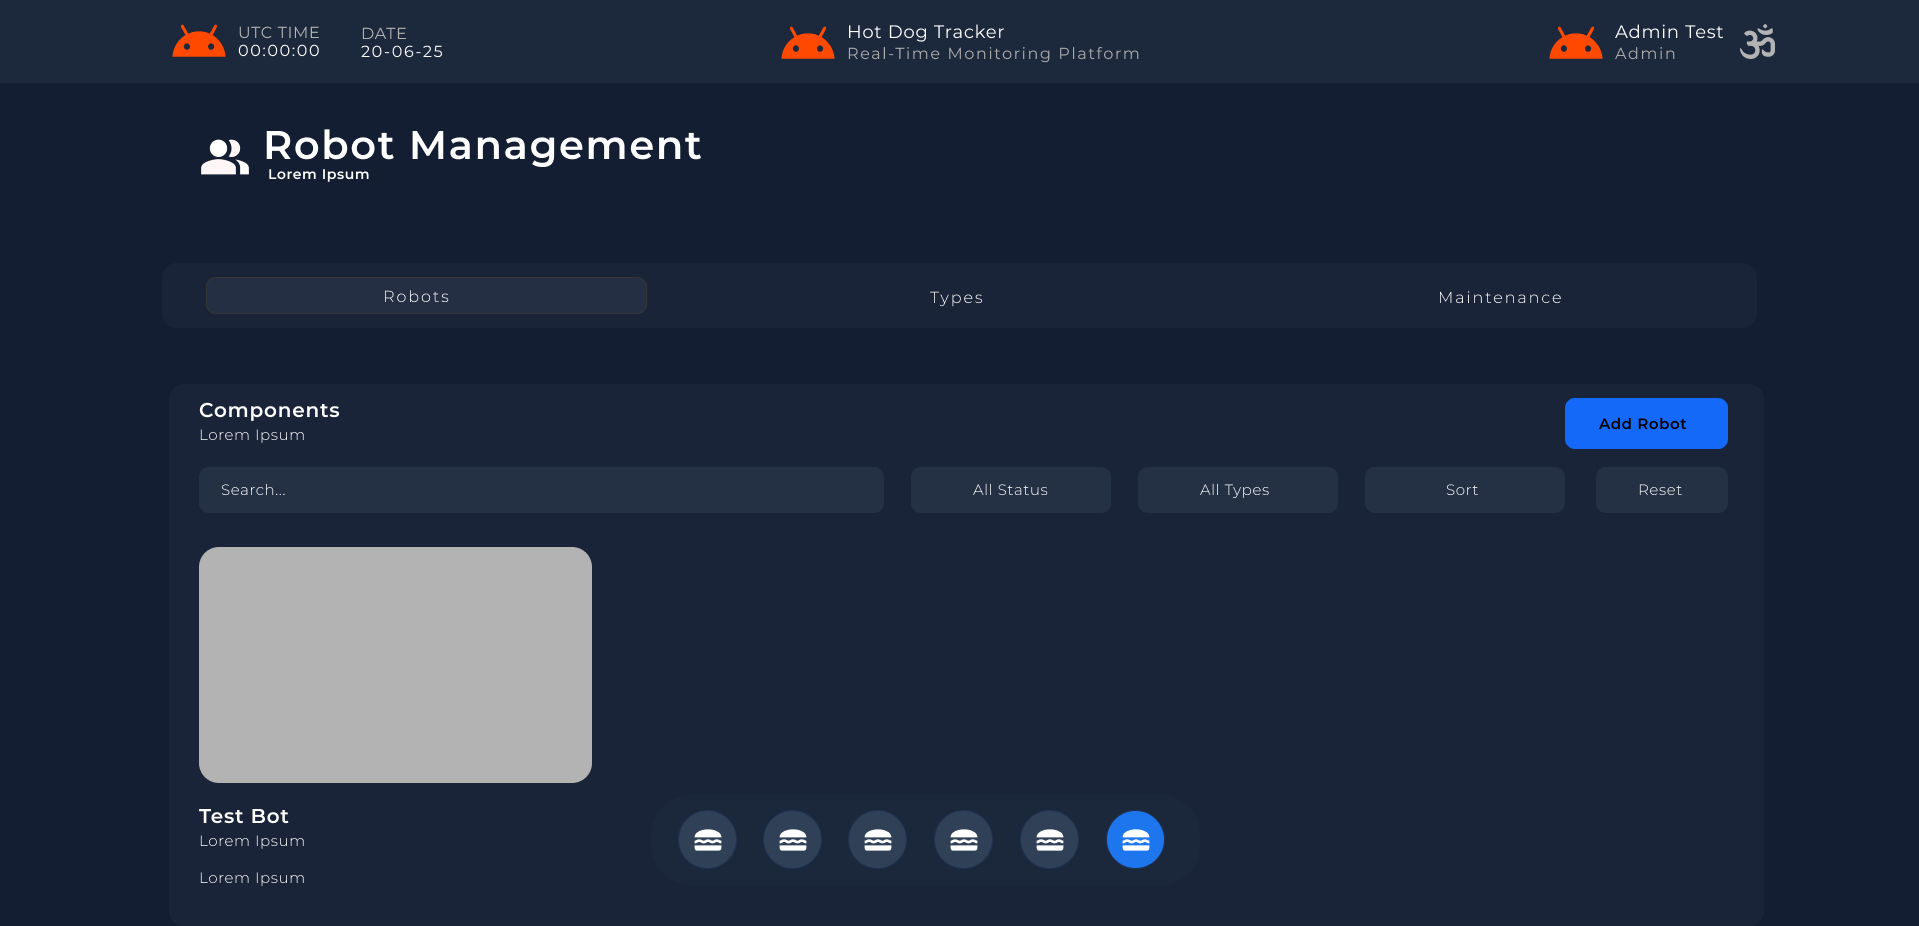
\includegraphics[width=0.8\textwidth]{gambar/bab3/robot-ui.png}
  \caption{Desain halaman manajemen robot \emph{control station}}
  \label{fig:control-station-robot-robot}
  \footnotesize{\textbf{Sumber:} Dokumentasi Pribadi}
\end{figure}

\begin{figure}[H]
  \centering
  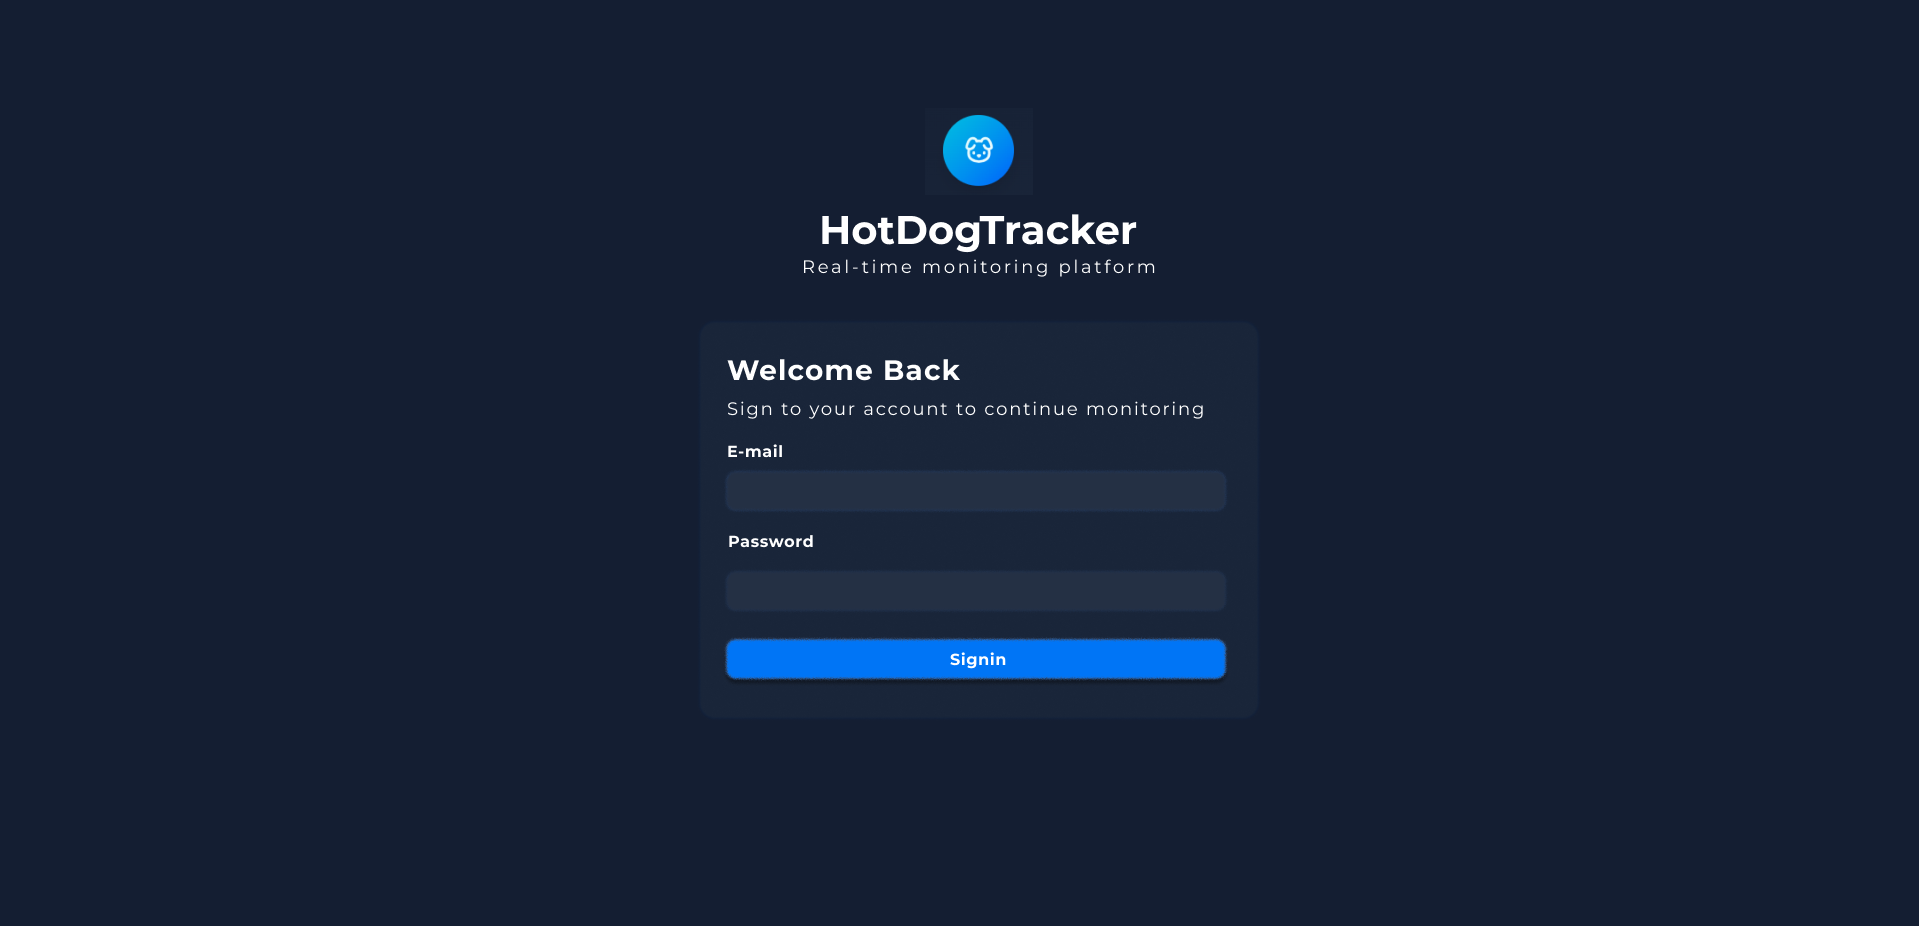
\includegraphics[width=0.8\textwidth]{gambar/bab3/auth-ui.png}
  \caption{Desain halaman manajemen komponen gardu \emph{control station}}
  \label{fig:control-station-robot-subtantion}
  \footnotesize{\textbf{Sumber:} Dokumentasi Pribadi}
\end{figure}


\begin{figure}[H]
  \centering
  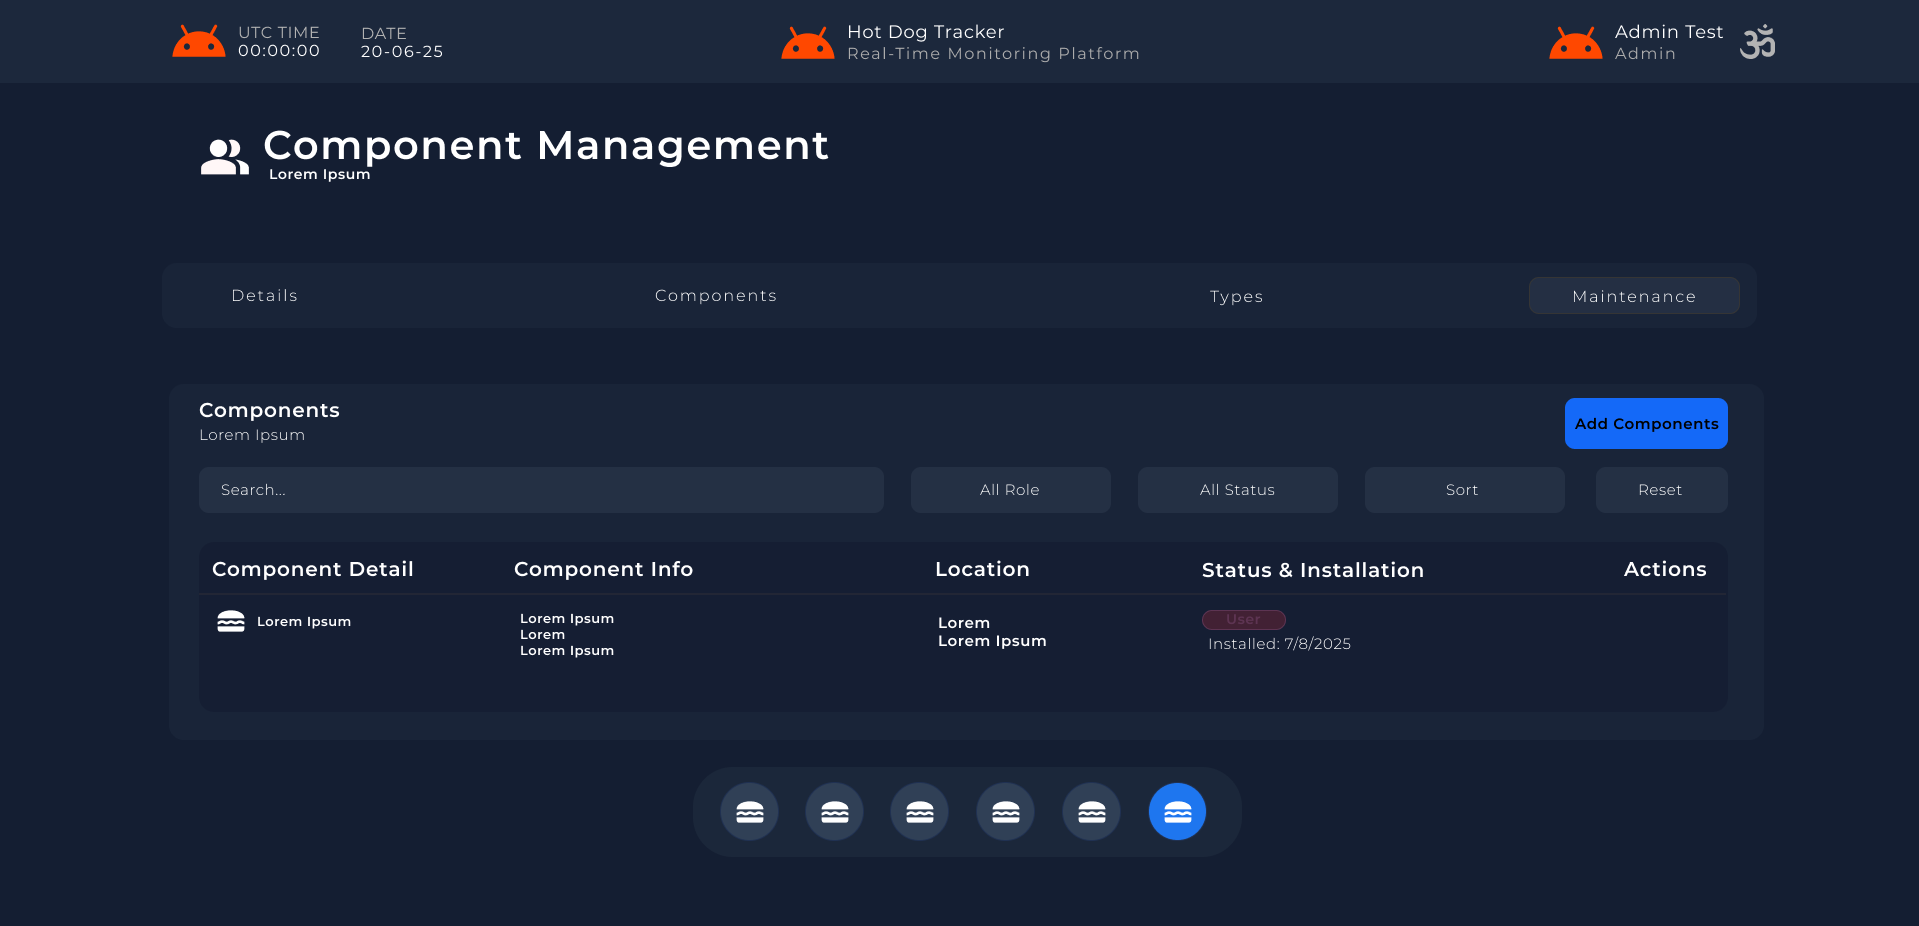
\includegraphics[width=0.8\textwidth]{gambar/bab3/component-ui.png}
  \caption{Desain halaman manajemen komponen patrol \emph{control station}}
  \label{fig:control-station-robot-patrol}
  \footnotesize{\textbf{Sumber:} Dokumentasi Pribadi}
\end{figure}

\begin{figure}[H]
  \centering
  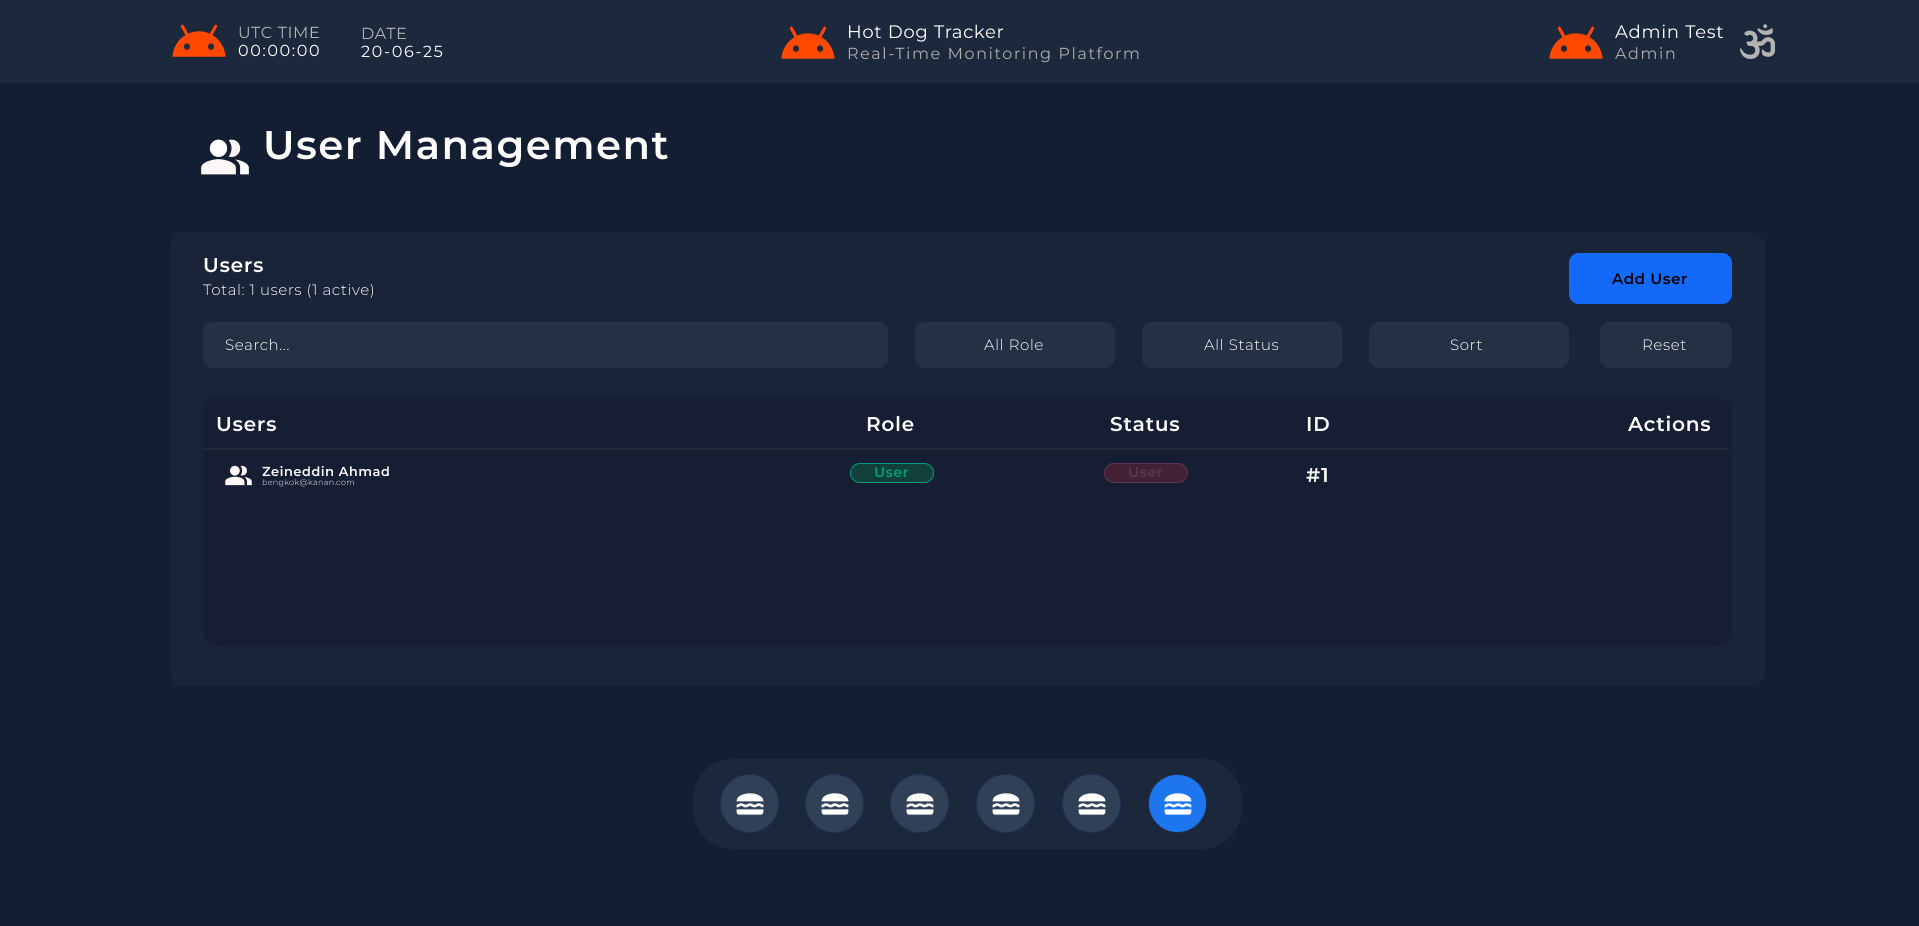
\includegraphics[width=0.8\textwidth]{gambar/bab3/user-ui.png}
  \caption{Desain halaman manajemen komponen user \emph{control station}}
  \label{fig:control-station-robot-user}
  \footnotesize{\textbf{Sumber:} Dokumentasi Pribadi}
\end{figure}

\begin{figure}[H]
  \centering
  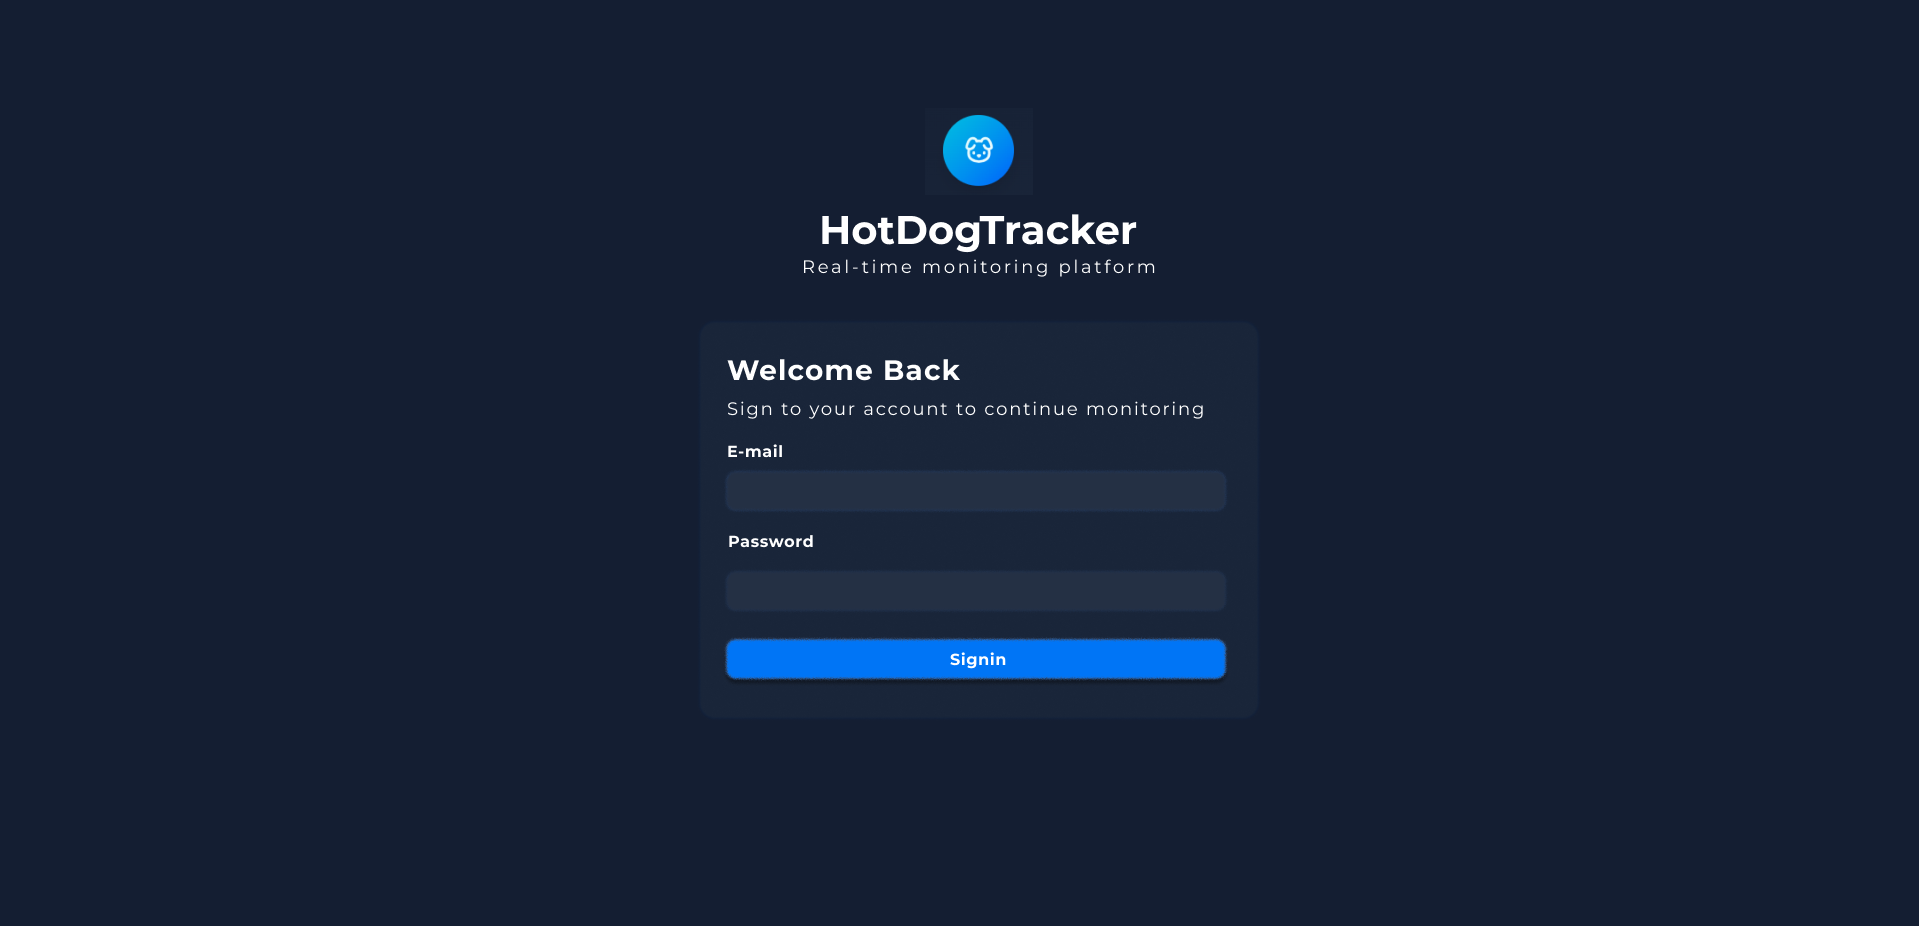
\includegraphics[width=0.8\textwidth]{gambar/bab3/auth-ui.png}
  \caption{Desain halaman hasil deteksi overheat \emph{control station}}
  \label{fig:control-station-robot-feature}
  \footnotesize{\textbf{Sumber:} Dokumentasi Pribadi}
\end{figure}


\begin{figure}[H]
  \centering
  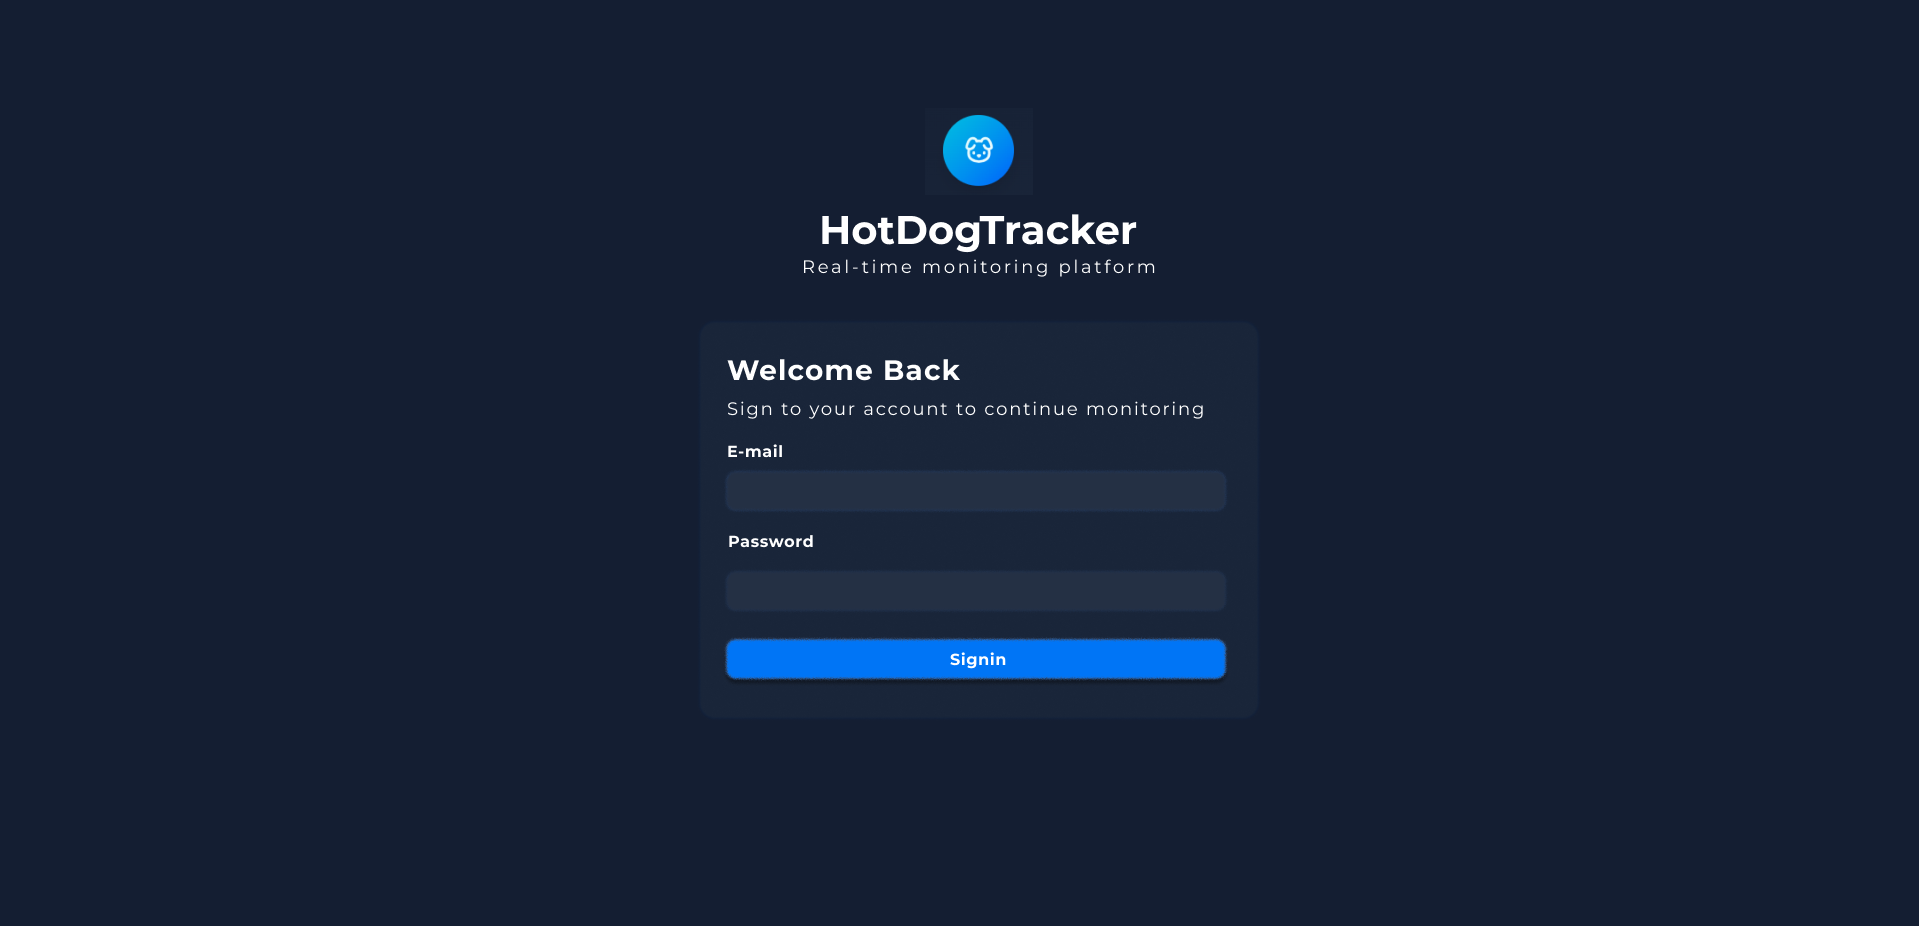
\includegraphics[width=0.8\textwidth]{gambar/bab3/auth-ui.png}
  \caption{Desain halaman \emph{configurasi system control station}}
  \label{fig:control-station-robot-setting}
  \footnotesize{\textbf{Sumber:} Dokumentasi Pribadi}
\end{figure}


\subsubsection{3.2.4.2 \emph{Physical data model design}}
\emph{Physical data model design} berfokus pada strukturisasi dan organisasi data yang akan dikelola oleh sistem. Ini meliputi definisi entitas data seperti data robot, komponen gardu, route, riwayat patroli, user, dan informasi konfigurasi sistem. Perancangan ini juga mencakup penetapan relasi antar entitas dan tipe data untuk memastikan integritas dan efisiensi penyimpanan serta pengambilan data. Adapun \emph{physical data model} yang digunakan dalam sistem ini dapat dilihat pada Gambar~\ref{fig:physical-data-model}.

\begin{figure}[H]
  \centering
  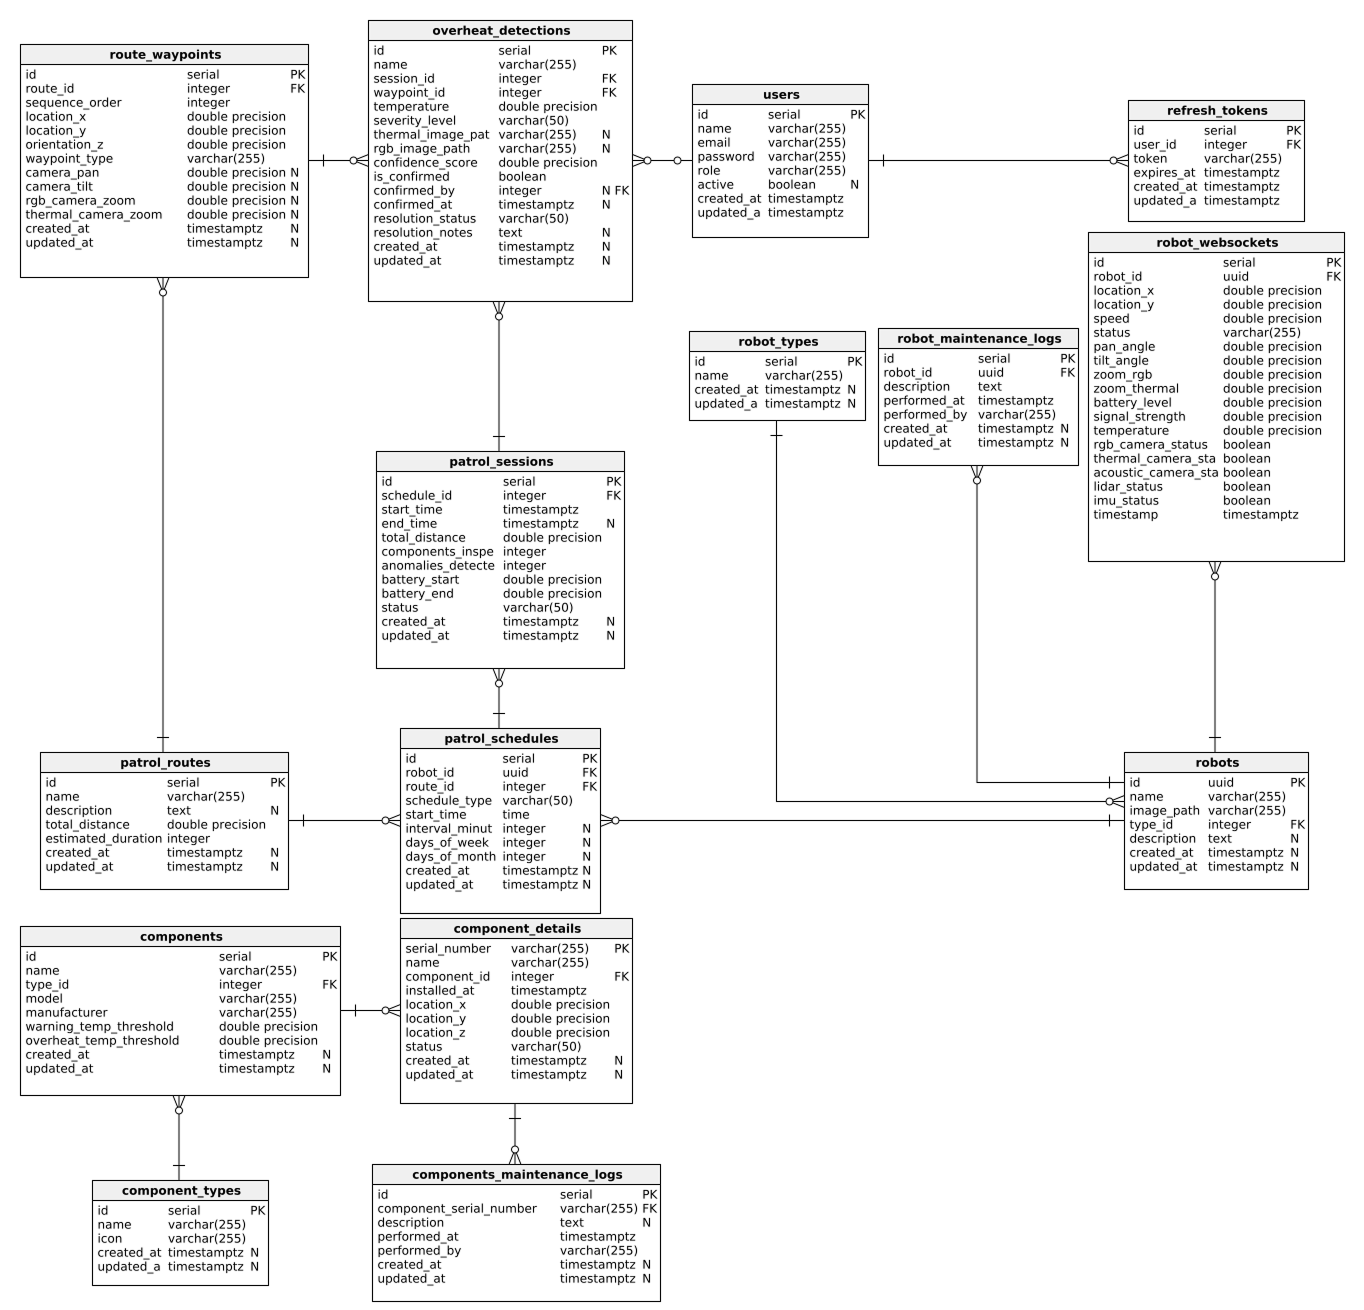
\includegraphics[width=0.87\textwidth]{gambar/bab3/pdm.png}
  \caption{\emph{Physical Data Model} \emph{Control Station}}
  \label{fig:physical-data-model}
  \footnotesize{\textbf{Sumber:} Dokumentasi Pribadi}
\end{figure}

\sloppy
Dari \emph{physical data model} \ref{fig:physical-data-model}, terlihat adanya entitas utama seperti \texttt{robots}, \texttt{patrol\_routes}, \texttt{patrol\_schedules}, dan \texttt{patrol\_sessions} yang merepresentasikan proses penjadwalan dan pelaksanaan patroli robot. Entitas \texttt{components} dan \texttt{component\_details} digunakan untuk menyimpan data komponen gardu yang dimonitor, termasuk jenis, lokasi pemasangan, serta parameter ambang batas suhu abnormal. Informasi jenis komponen disimpan dalam entitas \texttt{component\_types}. Deteksi suhu berlebih atau potensi overheat direkam dalam tabel \texttt{overheat\_detections}, yang terhubung dengan sesi patroli dan data komponen terkait. Posisi dan status robot secara waktu nyata dikelola melalui entitas \texttt{robot\_websockets}, yang mencatat data seperti posisi, arah, status sensor, dan kekuatan sinyal. Sistem ini juga mencakup manajemen pengguna dengan tabel \texttt{users} dan \texttt{refresh\_tokens} untuk kebutuhan autentikasi dan otorisasi. Informasi jenis robot disimpan dalam tabel \texttt{robot\_types}. Relasi antar tabel dirancang untuk mendukung integritas data dan efisiensi operasional sistem pemantauan dan pengendalian robot.

\subsubsection{3.2.4.3 \emph{Use case diagram}}
\emph{Use case diagram} digunakan untuk menggambarkan interaksi antara pengguna (aktor) dengan sistem. Diagram ini membantu dalam memahami kebutuhan fungsional sistem dan bagaimana pengguna akan berinteraksi dengan berbagai fitur yang disediakan. Berikut adalah \emph{use case diagram} yang menggambarkan interaksi antara pengguna dengan sistem \emph{control station}:

\begin{figure}[H]
  \centering
  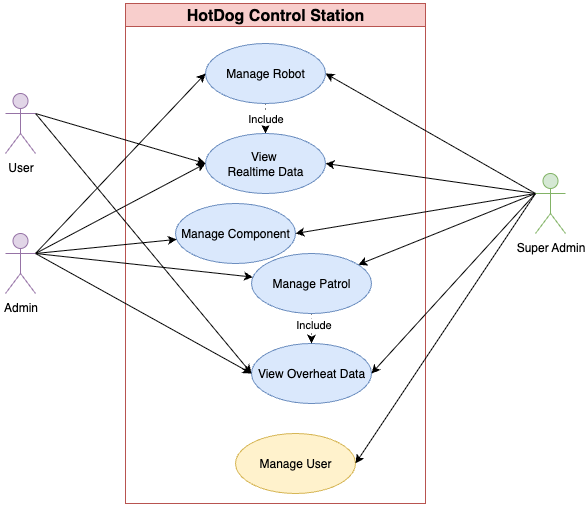
\includegraphics[width=0.8\textwidth]{gambar/bab3/usecase.png}
  \caption{\emph{Use Case Diagram} \emph{Control Station}}
  \label{fig:use-case-diagram}
  \footnotesize{\textbf{Sumber:} Dokumentasi Pribadi}
\end{figure}

Pada diagram tersebut terdapat tiga aktor, yaitu \texttt{User}, \texttt{Admin}, dan \texttt{Super Admin}, yang masing-masing memiliki tingkat akses berbeda terhadap sistem. Aktor \texttt{User} hanya memiliki akses untuk melihat data posisi dan data \emph{realtime} robot melalui fitur \texttt{View Realtime Data}, serta melihat data suhu berlebih melalui fitur \texttt{View Overheat Data}. Aktor \texttt{Admin} memiliki akses lebih luas, mencakup pengelolaan robot, komponen, dan jadwal patroli, serta melihat data anomali suhu, namun tidak memiliki wewenang untuk mengelola pengguna. Akses penuh terhadap seluruh fitur sistem, termasuk \texttt{Manage User}, hanya dimiliki oleh aktor \texttt{Super Admin}. Fitur \texttt{View Realtime Data} merupakan bagian dari \texttt{Manage Robot}, sedangkan \texttt{View Overheat Data} termasuk dalam \texttt{Manage Patrol}. Diagram ini menggambarkan batasan interaksi dan hak akses masing-masing aktor terhadap sistem \emph{Control Station}.


\section{Implementasi Sistem}
\sloppy
Implementasi sistem dilakukan dengan meimplementasikan rancangan yang telah dibuat pada tahap sebelumnya. Proses implementasi ini mencakup pengembangan perangkat lunak robot, integrasi perangkat keras, serta pengembagan sistem \emph{control station}.

\subsection{Implementasi Sistem \emph{Electrical}}
Implementasi sistem elektrikal dilakukan dengan mengintegrasikan komponen-komponen tambahan ke dalam robot yang telah ada. Proses ini meliputi pemasangan kamera termal, router nirkabel, dan perangkat \emph{switch} jaringan. Pemasangan dilakukan dengan memperhatikan skema distribusi daya yang telah dirancang sebelumnya, sehingga seluruh komponen dapat beroperasi dengan baik tanpa memerlukan sumber daya eksternal tambahan. Catu daya 24~VDC disuplai langsung dari port daya pada \emph{navigation host} robot seperti pada Gambar~\ref{fig:int-control-port}. 

\begin{figure}[H]
  \centering
  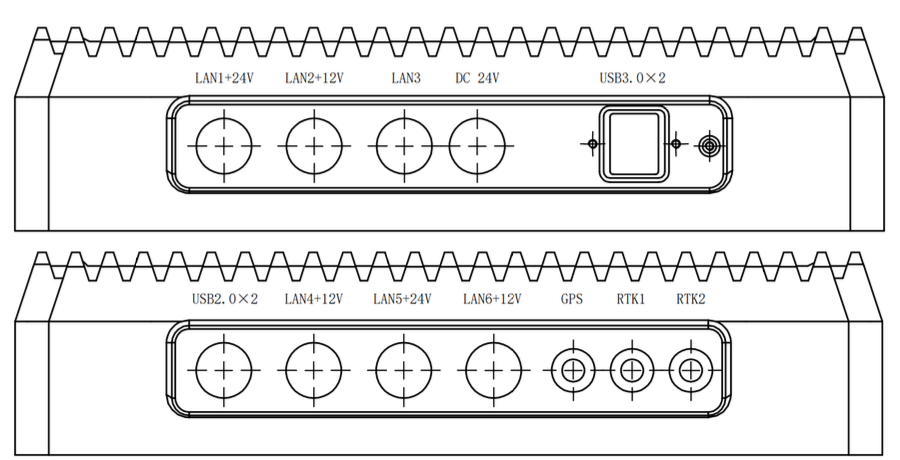
\includegraphics[width=0.8\textwidth]{gambar/bab3/int-control-port.png}
  \caption{Port pada \emph{Navigation Host} Robot  Tampak depan (atas) dan belakang (bawah)}
  \label{fig:int-control-port}
  \footnotesize{\textbf{Sumber:} Jueying X30 Pro Application Manual}
\end{figure}

Berdasarkan gambar di atas, dapat diketahui bahwa robot memiliki catu daya 24~VDC yang dapat digunakan untuk menyuplai perangkat tambahan. Berdasarkan data spesifikasi dari Deep Robotics X30 Pro, daya maksimum yang dapat disuplai oleh satu port 24~V adalah 240~W, atau dengan arus maksimum sebesar 10~A  Sementara itu perangkat tambahan yang digunakan terdiri dari:
\begin{enumerate}
  \item Kamera termal Hikvision HM-TD5528T-15/W dengan \emph{power consumption}  sebesar 20~W,
  \item Router nirkabel Doublecom DB6000FR-ANS dengan \emph{maximum power consumption} kurang dari 9~W,
  \item \emph{Switch} Moxa EDS-205  dengan \emph{input current 0.12~A} pada 24~VDC, sehingga daya yang dibutuhkan adalah 2.88~W
\end{enumerate}


Beradaskan data diatas total daya yang dibutuhkan oleh perangkat tambahan adalah:
\[
P_{\text{total}} = 20~W + 9~W + 2{,}88~W = 31{,}88~W
\]

Jika tegangan yang digunakan konstan 24~V, maka arus yang digunakan oleh perangkat tambahan adalah:
\[
I = \frac{P_{\text{total}}}{V} = \frac{31{,}88~W}{24~V} \approx 1{,}33~A
\]

Persentase penggunaan terhadap kapasitas maksimum port adalah:
\[
\text{Daya (\%P):} \quad \frac{31{,}88}{240} \times 100\% \approx 13{,}283333333\%
\]

Dengan demikian, total konsumsi daya dan arus perangkat tambahan hanya sekitar 13{,}3\% dari kapasitas maksimum port 24~V, sehingga masih berada dalam batas aman dan tidak membebani sistem catu daya robot. Selain sistem catu daya, implementasi ini juga mencakup konfigurasi komunikasi perangkat tambahan agar dapat diakses oleh robot. Dalam implementasinya, perangkat \emph{switch} Doublecom yang terpasang pada robot akan dihubungkan dengan perangkat \emph{switch} eksternal yang juga terhubung dengan kamera termal. Kedua \emph{switch} ini selanjutnya dihubungkan ke port jaringan pada robot. Seluruh perangkat dikonfigurasi dalam jaringan lokal dengan skema alamat IP yang sama, yaitu 192.168.1.\texttt{x}, sehingga dapat saling berkomunikasi tanpa melalui jaringan publik. Kamera termal, yang telah diatur menggunakan alamat IP statis 192.168.1.64, akan berada dalam satu segmen jaringan dengan router dan robot, memungkinkan akses data secara langsung melalui jalur Ethernet. Robot yang telah terintegrasi dengan komponen tambahan dapat dilihat pada gambar \ref{fig:sistem-elec-robot}


\begin{figure}[H]
  \centering
  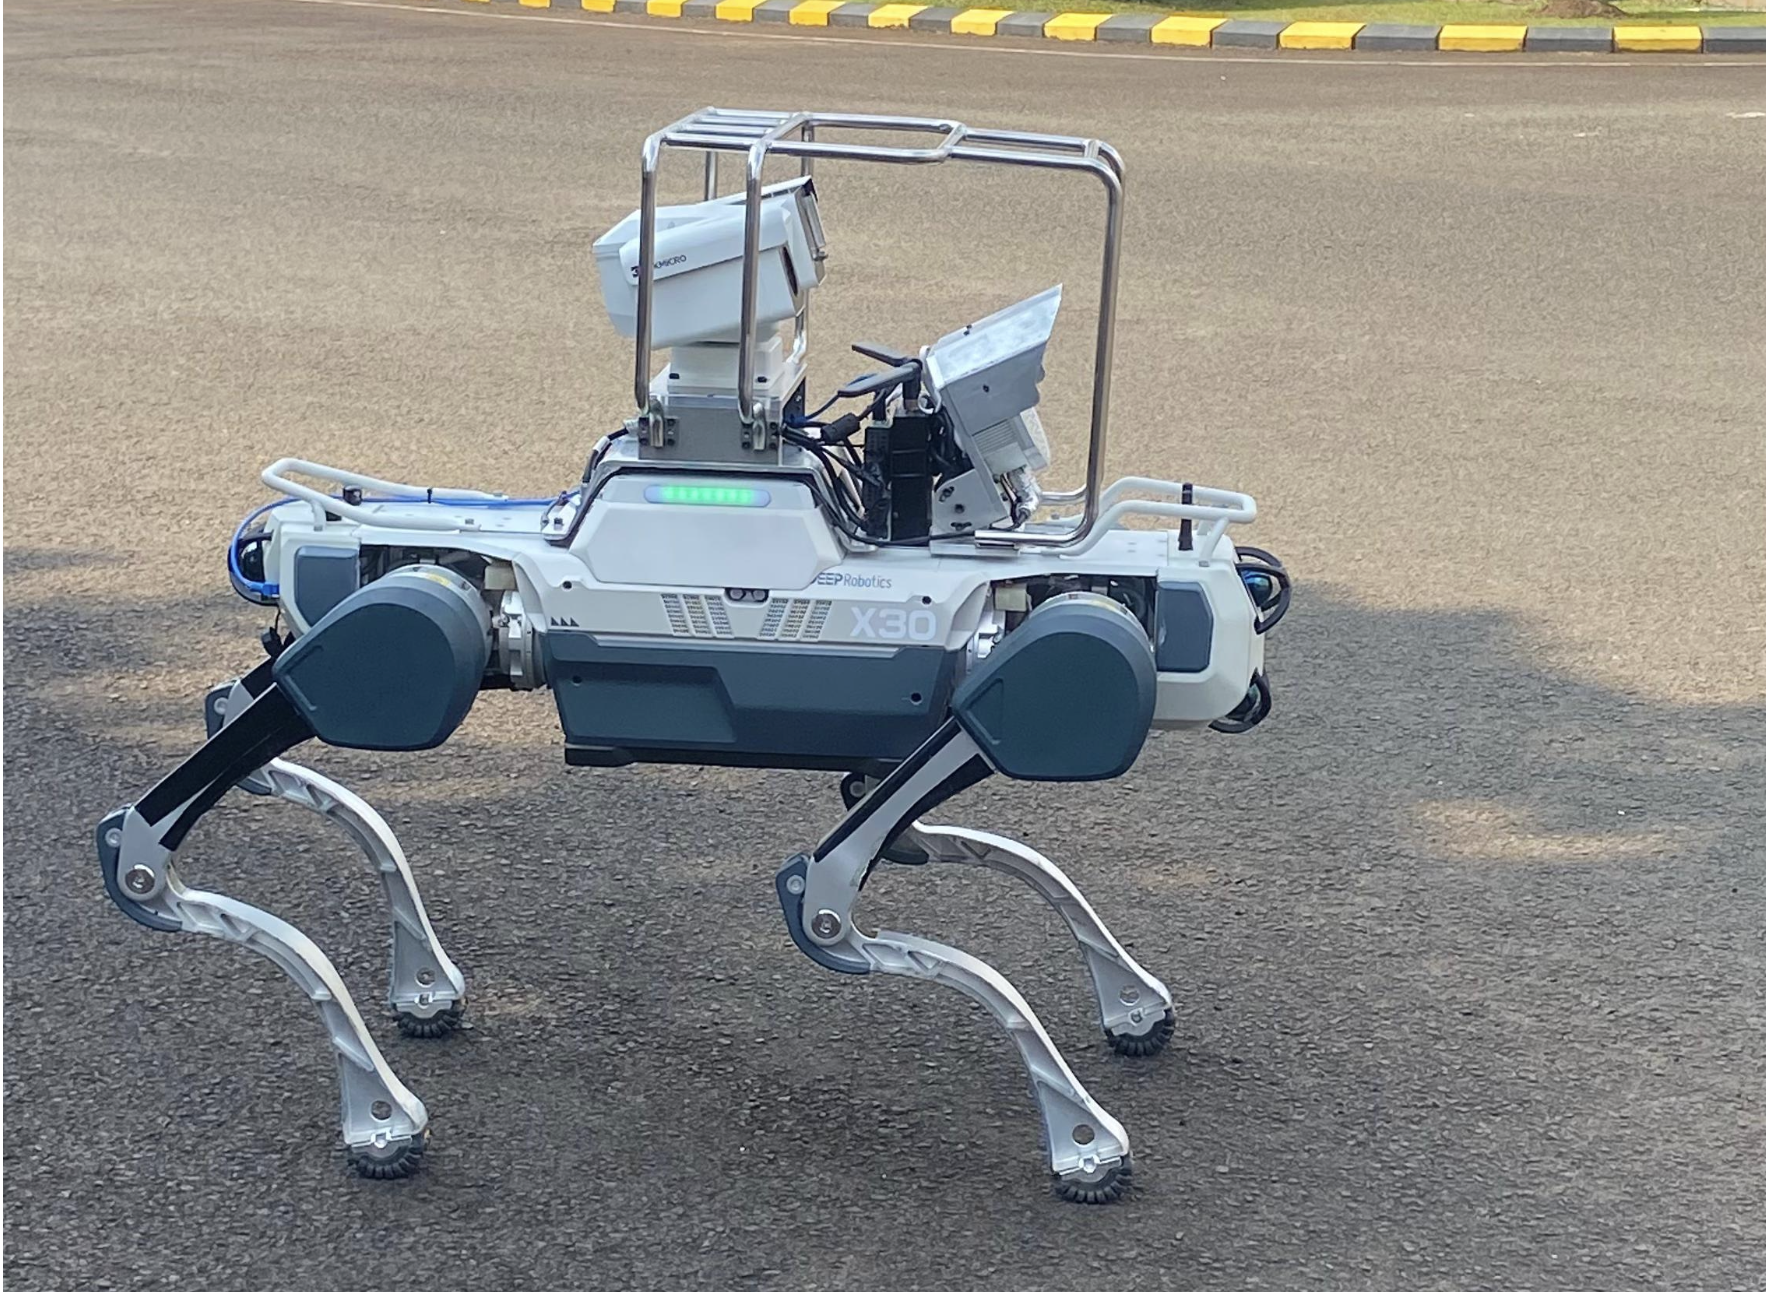
\includegraphics[width=0.8\textwidth]{gambar/bab3/impl-elec2.png}
  \caption{Integrasi robot dengan hardware external yang diperlukan}
  \label{fig:sistem-elec-robot}
  \footnotesize{\textbf{Sumber:} Dokumentasi pribadi}
\end{figure}

\subsection{Implementasi sistem \emph{computer vision}}
Pada tahap implementasi sistem \emph{computer vision}, dilakukan beberapa langkah utama yang mencakup pembuatan dataset, pelatihan model deteksi objek, konversi model ke format \emph{OpenVINO}, dan inferensi model untuk mendeteksi objek serta menganalisis suhu komponen gardu induk. Proses ini bertujuan untuk mengidentifikasi komponen gardu induk yang mengalami kondisi \emph{overheat} berdasarkan citra termal yang diambil oleh kamera termal yang terpasang pada robot.


\subsubsection{3.3.2.1 Pembuatan Dataset}
Dataset citra termal yang digunakan dalam penelitian ini berasal dari dua sumber utama. Dataset pertama diperoleh dari repositori publik \emph{Roboflow Universe}, yang menyediakan citra termal berbagai komponen gardu induk, seperti \emph{arrester}, \emph{breaker}, \emph{bushing}, \emph{clamp}, \emph{conservator}, \emph{current transformer}, \emph{disconnector}, \emph{heat sink}, \emph{insulator}, dan \emph{transformer}. Dataset kedua dikumpulkan secara langsung dari GITET (Gardu Induk Tegangan Ekstra Tinggi) PLN Gandul melalui proses perekaman video menggunakan kamera termal robot. Video hasil perekaman tersebut kemudian diunggah ke platform \emph{Roboflow}, yang secara otomatis mengkonversi video menjadi kumpulan citra (frame) individual. Citra-citra inilah yang selanjutnya digunakan sebagai dasar proses anotasi. Setiap komponen pada citra termal diberi label sesuai kelasnya, seperti \emph{current transformer}, \emph{circuit breaker}, maupun PMT (Pemutus tegangan gardu) seperti ditunjukkan pada Gambar~\ref{fig:dataset-annotated}. 
\begin{figure}[H]
  \centering
  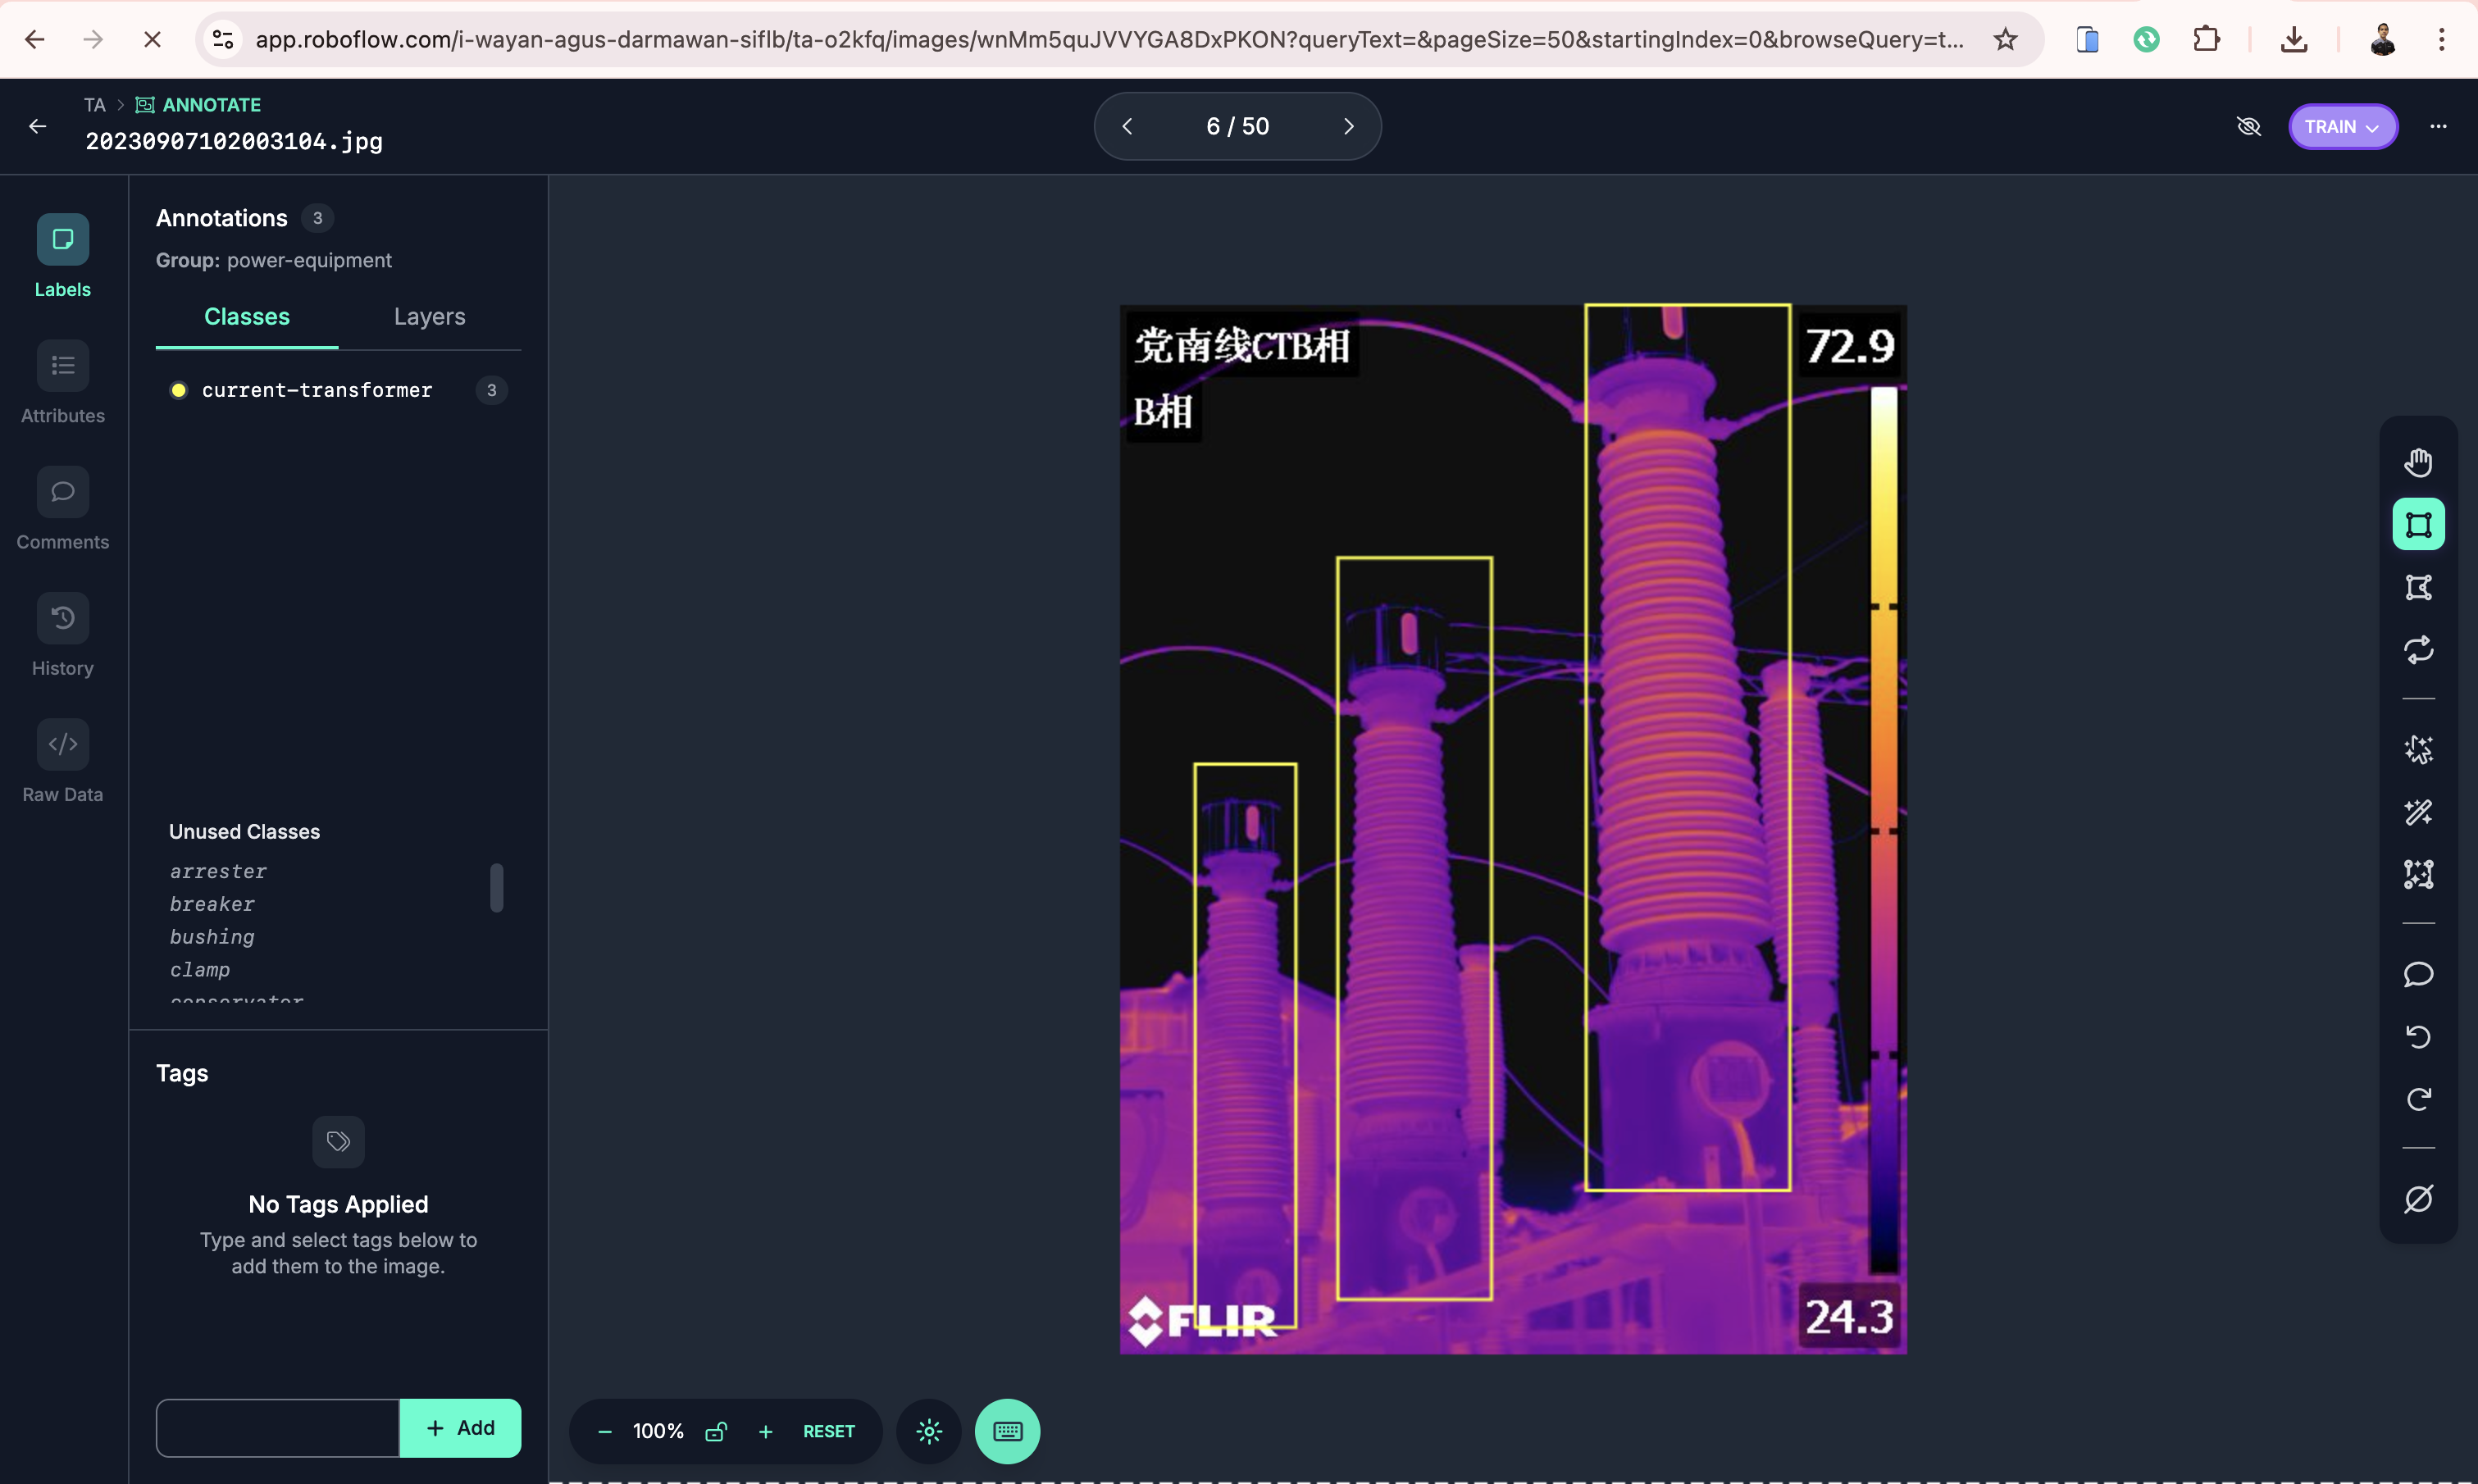
\includegraphics[width=0.7\textwidth]{gambar/bab3/dataset-anotated.png}
  \caption{Labeling dataset citra termal pada \emph{Roboflow}}
  \label{fig:dataset-annotated}
  \footnotesize{\textbf{Sumber:} Dokumentasi Pribadi}
  \end{figure}
  
Proses anotasi ini krusial untuk memastikan model mampu mengenali dan mengklasifikasikan berbagai komponen gardu induk dengan akurat berdasarkan karakteristik citra termal. Dataset kemudian di bagi menjadi tiga bagian: data pelatihan, data validasi, dan data uji. Proporsi pembagian dataset adalah 70\% untuk pelatihan, 20\% untuk validasi, dan 10\% untuk pengujian. Pembagian ini bertujuan untuk memastikan model dapat belajar dengan baik dari data yang tersedia, serta menghindari overfitting pada saat pelatihan.

\subsubsection{3.3.2.2 \emph{Preprocessing} Dataset}
Setelah dataset citra termal dikumpulkan dan dianotasi, langkah selanjutnya adalah melakukan proses \emph{preprocessing} terhadap data tersebut. Pada penelitian ini, \emph{preprocessing} dilakukan dengan mengubah ukuran citra agar sesuai dengan format input yang dibutuhkan oleh model deteksi objek. Ukuran citra yang digunakan adalah 640$\times$480 piksel, yang merupakan standar umum untuk banyak arsitektur model deteksi seperti YOLO. Penyesuaian ukuran ini bertujuan untuk memastikan konsistensi data masukan, mempercepat proses pelatihan, serta meningkatkan performa dan akurasi model.


\subsubsection{3.3.2.3 \emph{Augmentasi} Data}
Untuk meningkatkan variasi data pelatihan dan mengurangi risiko \emph{overfitting}, dilakukan proses \emph{augmentasi} pada dataset citra termal. Proses ini menjadi sangat penting mengingat keterbatasan dalam pengambilan data lapangan secara langsung. Gardu induk merupakan objek vital nasional yang memiliki akses terbatas dan prosedur keamanan yang ketat, sehingga tidak memungkinkan untuk melakukan pengambilan data dalam jumlah besar secara bebas dan berulang. Oleh karena itu, augmentasi data digunakan untuk mensimulasikan berbagai kondisi nyata tanpa harus menambah data mentah secara langsung. Teknik augmentasi yang diterapkan meliputi \emph{Gaussian blur} untuk menyimulasikan kondisi citra buram akibat pergerakan atau gangguan fokus, penyesuaian tingkat kecerahan (\emph{brightness adjustment}) dan rona warna (\emph{hue adjustment}) untuk merepresentasikan variasi pencahayaan dan spektrum inframerah, serta \emph{horizontal flip} untuk menambah keragaman perspektif tampilan komponen. Sementara itu, \emph{vertical flip} tidak digunakan karena orientasi vertikal komponen gardu seperti trafo dan pemutus arus tidak mungkin berubah dalam kondisi nyata. Dengan pendekatan ini, model diharapkan tetap mampu belajar secara optimal meskipun jumlah data asli dari lapangan terbatas.

\subsubsection{3.3.2.4 Pelatihan Model \emph{YOLOv8}}

Model \emph{YOLOv8} dilatih menggunakan dataset citra termal yang telah melalui proses anotasi, \emph{preprocessing} dan \emph{augmentasi}. Selama proses pelatihan, dilakukan pengaturan terhadap beberapa \emph{hyperparameter} utama, yaitu \emph{batch size}, jumlah \emph{epoch}, dan algoritma \emph{optimizer}, guna memperoleh performa model yang optimal. Nilai \emph{batch size} yang digunakan dalam eksperimen adalah 2, 4, dan 8, sedangkan jumlah \emph{epoch} yang diuji bervariasi mulai dari 50, 100, 150, hingga 200. Untuk algoritma optimisasi, dilakukan perbandingan antara \emph{Stochastic Gradient Descent} (SGD) dan \emph{Adam Optimizer} guna melihat pengaruhnya terhadap kecepatan konvergensi dan stabilitas model.  Setelah proses pelatihan selesai, model dievaluasi menggunakan dataset uji yang telah dipisahkan sebelumnya untuk memastikan hasil validasi yang objektif dan menghindari risiko \emph{overfitting}. Evaluasi ini dilakukan dengan mengukur metrik seperti \emph{precision}, \emph{recall}, dan \emph{mAP (mean Average Precision)} guna mengetahui seberapa baik model dapat mendeteksi komponen gardu induk berdasarkan citra termal.


\subsubsection{3.3.2.5 Konversi ke \emph{OpenVINO}}
Setelah model \emph{YOLOv8} dilatih dan tervalidasi, tahap berikutnya adalah melakukan konversi ke format \emph{OpenVINO (Open Visual Inference and Neural Network Optimization)}. Konversi ini bertujuan untuk mengoptimalkan proses inferensi model agar dapat dijalankan secara efisien pada perangkat keras dengan sumber daya terbatas, khususnya yang berbasis CPU.

Dalam penelitian ini, sistem inferensi dirancang untuk dijalankan pada perangkat dengan prosesor Intel, sehingga penggunaan \emph{OpenVINO} menjadi pilihan ideal. \emph{OpenVINO} merupakan toolkit yang dikembangkan oleh Intel untuk mempercepat kinerja model \emph{deep learning} pada arsitektur CPU, GPU, dan VPU Intel. Dengan melakukan konversi model ke format \emph{Intermediate Representation (IR)} yang terdiri dari file \texttt{.xml} dan \texttt{.bin}, model dapat dieksekusi lebih ringan dan cepat, tanpa memerlukan akselerator eksternal seperti GPU.

\subsubsection{3.3.2.6 Inferensi Komponen}

Proses inferensi komponen dilakukan setelah robot tiba pada titik \emph{waypoint} tertentu dan mengambil citra termal menggunakan kamera yang terpasang. Citra tersebut kemudian diproses oleh model deteksi objek \emph{YOLOv8} yang telah dilatih dan dikonversi ke dalam format \emph{OpenVINO} agar dapat berjalan secara efisien di perangkat dengan prosesor Intel. Model ini melakukan deteksi pada citra termal untuk mengidentifikasi dan mengklasifikasikan komponen gardu induk seperti \emph{current transformer}, \emph{circuit breaker}, \emph{bushing}, dan komponen lainnya.

Hasil inferensi berupa koordinat \emph{bounding box} dan label kelas dari masing-masing objek yang terdeteksi. Informasi ini digunakan untuk menentukan area citra yang akan dianalisis lebih lanjut, khususnya dalam konteks pemantauan suhu untuk mendeteksi potensi \emph{overheat}. Proses inferensi ini dilakukan secara waktu nyata (\emph{real-time}) dan menjadi dasar bagi tahapan analisis suhu komponen yang lebih spesifik.

\subsubsection{3.3.2.7 Klasifikasi Suhu Komponen}

Setelah komponen berhasil terdeteksi, tahap berikutnya adalah mengklasifikasikan suhu dari masing-masing komponen berdasarkan area \emph{bounding box}. Langkah pertama dalam proses ini adalah mengonversi citra termal ke dalam format \emph{grayscale}, di mana setiap nilai intensitas piksel (0--255) mewakili tingkat suhu relatif. Nilai-nilai ini kemudian dikonversi ke suhu aktual berdasarkan rentang suhu minimum dan maksimum yang dikonfigurasi pada kamera.

Rentang suhu tersebut diperoleh menggunakan protokol ISAPI melalui endpoint berikut:

\begin{center}
\texttt{GET /ISAPI/Image/channels/<ID>/tempRange}
\end{center}

Endpoint ini digunakan untuk membaca parameter suhu dari kanal tertentu pada kamera, di mana \texttt{<ID>} mengacu pada nomor kanal kamera termal. Jika permintaan berhasil, kamera akan mengembalikan data dalam format XML yang memuat nilai suhu minimum dan maksimum seperti berikut:

\begin{lstlisting}[language=XML]
<?xml version="1.0" encoding="utf-8"?>
<TempRange version="2.0" xmlns="http://www.isapi.org/ver20/XMLSchema">
    <mode>manual</mode>
    <temperatureUpperLimit>100</temperatureUpperLimit>
    <temperatureLowerLimit>20</temperatureLowerLimit>
</TempRange>
\end{lstlisting}

Nilai intensitas piksel dalam area \emph{bounding box} kemudian dikonversi ke suhu aktual (\(T\)) menggunakan rumus berikut:

\begin{equation}
T(x, y) = T_{\text{min}} + \left( \frac{I(x, y)}{255} \right) \times (T_{\text{max}} - T_{\text{min}})
\label{eq:suhu-piksel}
\end{equation}

\noindent
dengan keterangan:
\begin{itemize}
  \item \( T(x, y) \): suhu piksel pada posisi \((x, y)\),
  \item \( I(x, y) \): nilai intensitas piksel (0–255),
  \item \( T_{\text{min}} \), \( T_{\text{max}} \): suhu minimum dan maksimum dari kamera.
\end{itemize}

Setelah nilai suhu pada seluruh piksel dalam \emph{bounding box} dihitung, suhu rata-rata komponen ditentukan menggunakan persamaan:

\begin{equation}
T_{\text{avg}} = \frac{1}{N} \sum_{i=1}^{N} T(x_i, y_i)
\label{eq:rata-rata-suhu}
\end{equation}

\noindent
dengan \( N \) adalah jumlah total piksel dalam area komponen. Nilai suhu rata-rata ini kemudian dibandingkan dengan ambang batas tertentu untuk menentukan apakah suatu komponen mengalami suhu berlebih (\emph{overheat}).


